\documentclass[12pt,letterpaper,oneside]{book}
\usepackage{../../afitStyleFiles/afitThesis}
\usepackage[nolist]{acronym}
\usepackage{todo}
\usepackage{tabu}
\usepackage{makecell}
\renewcommand\theadfont{\bfseries}
\graphicspath{{../../Figures/}}
%% myFigures.tex
% A common file to store all figure definitions
%
% In preparing your thesis, one of the first things you should do is
% organize your figures.  Then, one of the last things you'll do is
% reorder your figures so they display where you want them to in the
% text.  Organizing figure definitions in a common files helps:
%
%   1. Write new figures using earlier examples.
%
%   2.  Isolate code and minimize the risk of introducing bugs in the
%   final editing process.  Trust me, moving around just one line of
%   code is easier.
%
%   3.  Reuse figures in other papers.  <=== the best reason!
%
% Note command names can not include numbers and special characters.
%
% To make the file more searchable, use naming conventions that map
% the graphics filename labSetup.jpg to the command name \figlabSetup to the
% figure label fig:labSetup.
% 

\newcommand{\figMpduFormat}{
	\begin{figure}[H]
		\begin{center}
			\makebox[\textwidth][c]{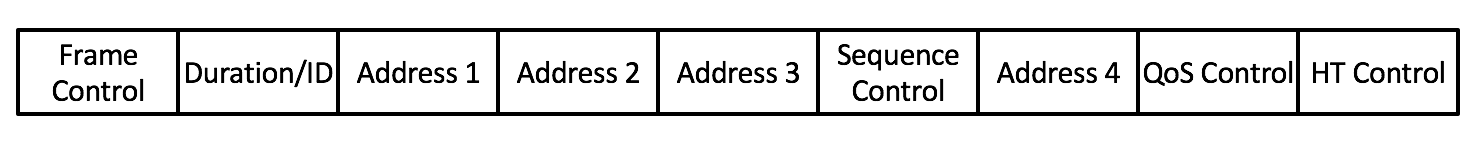
\includegraphics[width=\linewidth]{macHeader}}
			\caption{\ac{MPDU} format when using \ac{WPA}-2 \cite{802.11}}
			\label{fig:MpduFormat}
		\end{center}
		\vspace{-0.2 in}
	\end{figure}
}

\newcommand{\figMacHeader}{
	\begin{figure}[H]
		\begin{center}
			\makebox[\textwidth][c]{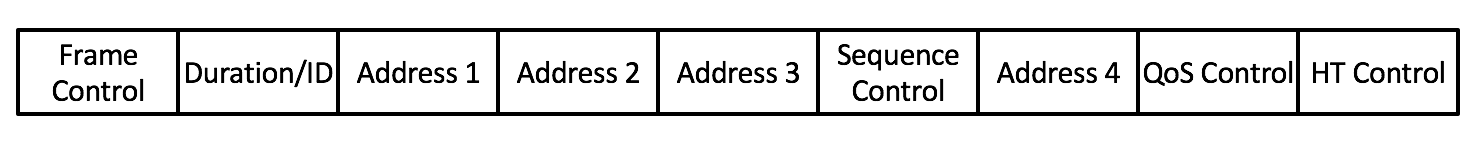
\includegraphics[width=\linewidth]{macHeader}}
			\caption{\ac{MAC} Header Frame Format \cite{802.11}}
			\label{fig:MacHeader}
		\end{center}
		\vspace{-0.2 in}
	\end{figure}
}

\newcommand{\figArchitecture}{\begin{figure}[H]
	\begin{center}
		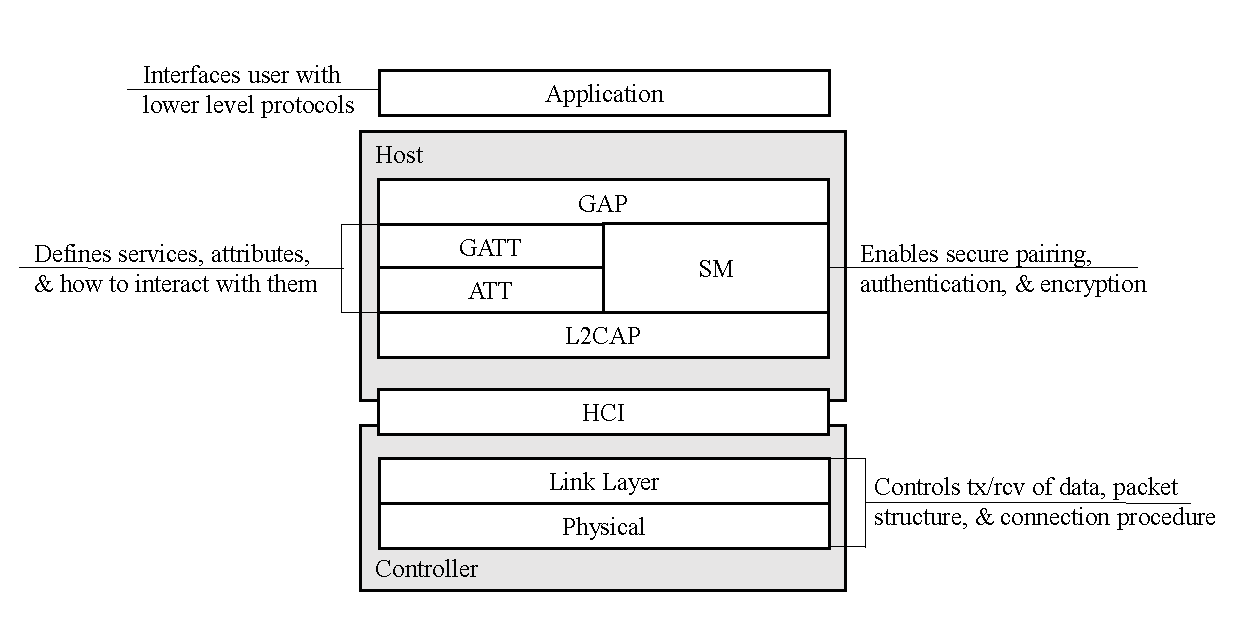
\includegraphics[width=4in]{architecture}
		\caption{The Bluetooth Low Energy Architecture}
		\label{fig:Architecture}
	\end{center}
	\vspace{-0.2 in}
\end{figure}
}

\newcommand{\figConnection}{\begin{figure}[H]
	\begin{center}
		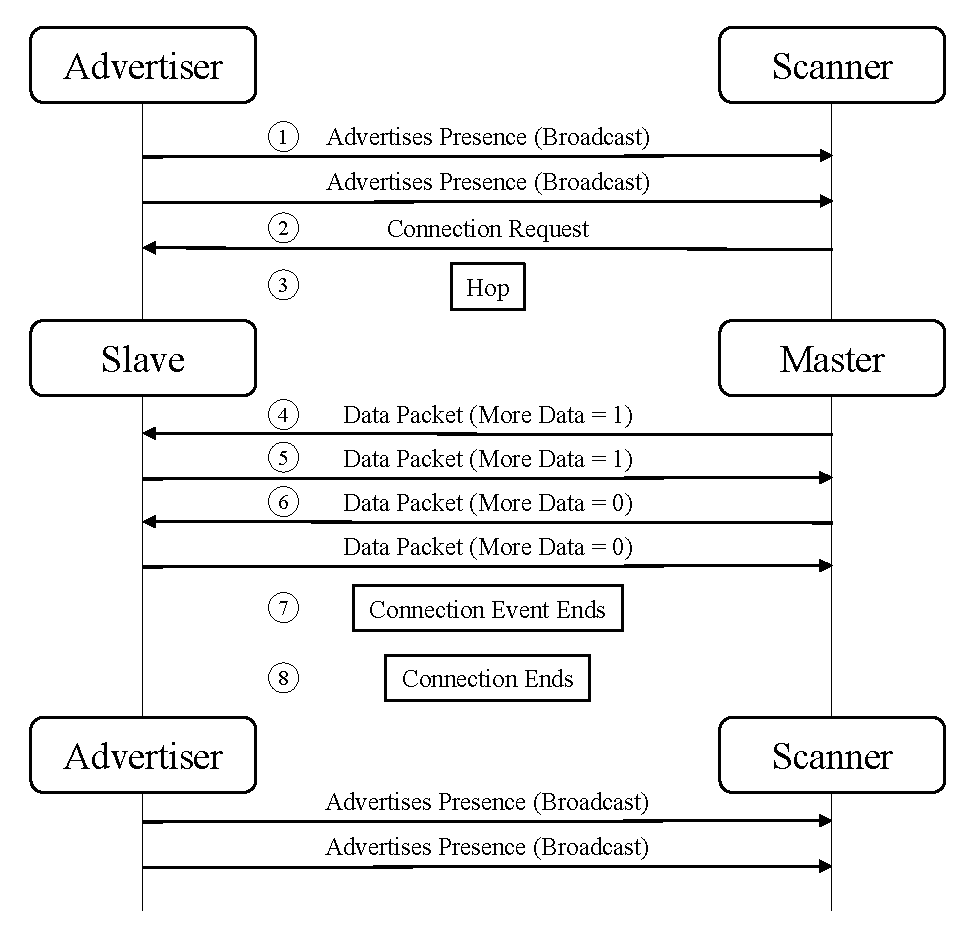
\includegraphics[width=4in]{connectionProcess}
		\caption{The \ac{BLE} Connection Process}
		\label{fig:Connection}
	\end{center}
	\vspace{-0.2 in}
\end{figure}
}

\newcommand{\figScanning}{\begin{figure}[H]
		\begin{center}
			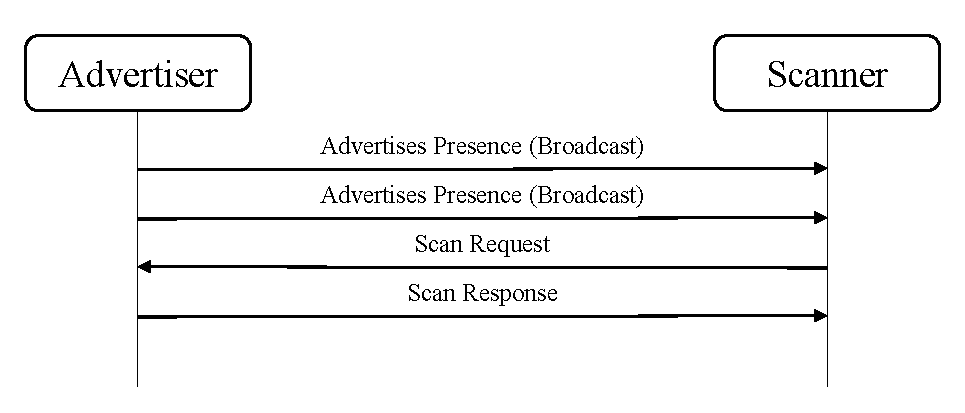
\includegraphics[width=4in]{activeScanning}
			\caption{Active Scanning Process}
			\label{fig:Scanning}
		\end{center}
		\vspace{-0.2 in}
	\end{figure}
}

\newcommand{\figChannel}{
	\begin{figure}[H]
		\begin{center}
			\includegraphics[width=5in]{channelMap}
			\caption{Bluetooth Low Energy channel mapping; darker channels represent advertisement channels}
			\label{fig:Channel}
		\end{center}
		\vspace{-0.2 in}
	\end{figure}
}

\newcommand{\figAccessPoint}{
	\begin{figure}[H]
		\begin{center}
			\makebox[\textwidth][c]{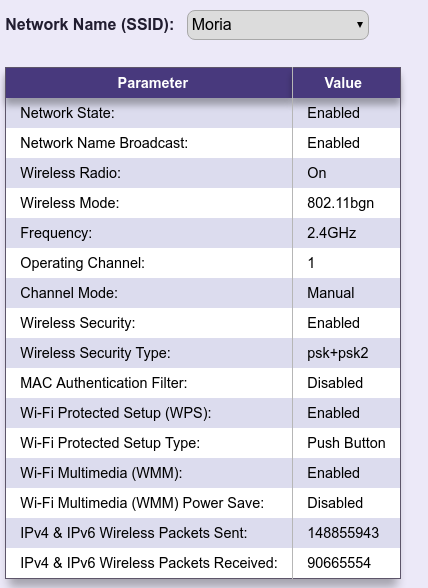
\includegraphics[width=2.5in]{accessPoint}}
			\caption{Prancing Pony Access Point Settings}
			\label{fig:AccessPoint}
		\end{center}
		\vspace{-0.2 in}
	\end{figure}
}

\newcommand{\figSystemDiagram}{
	\begin{figure}[h!]
		\begin{center}
			\centering
			\makebox[\textwidth][c]{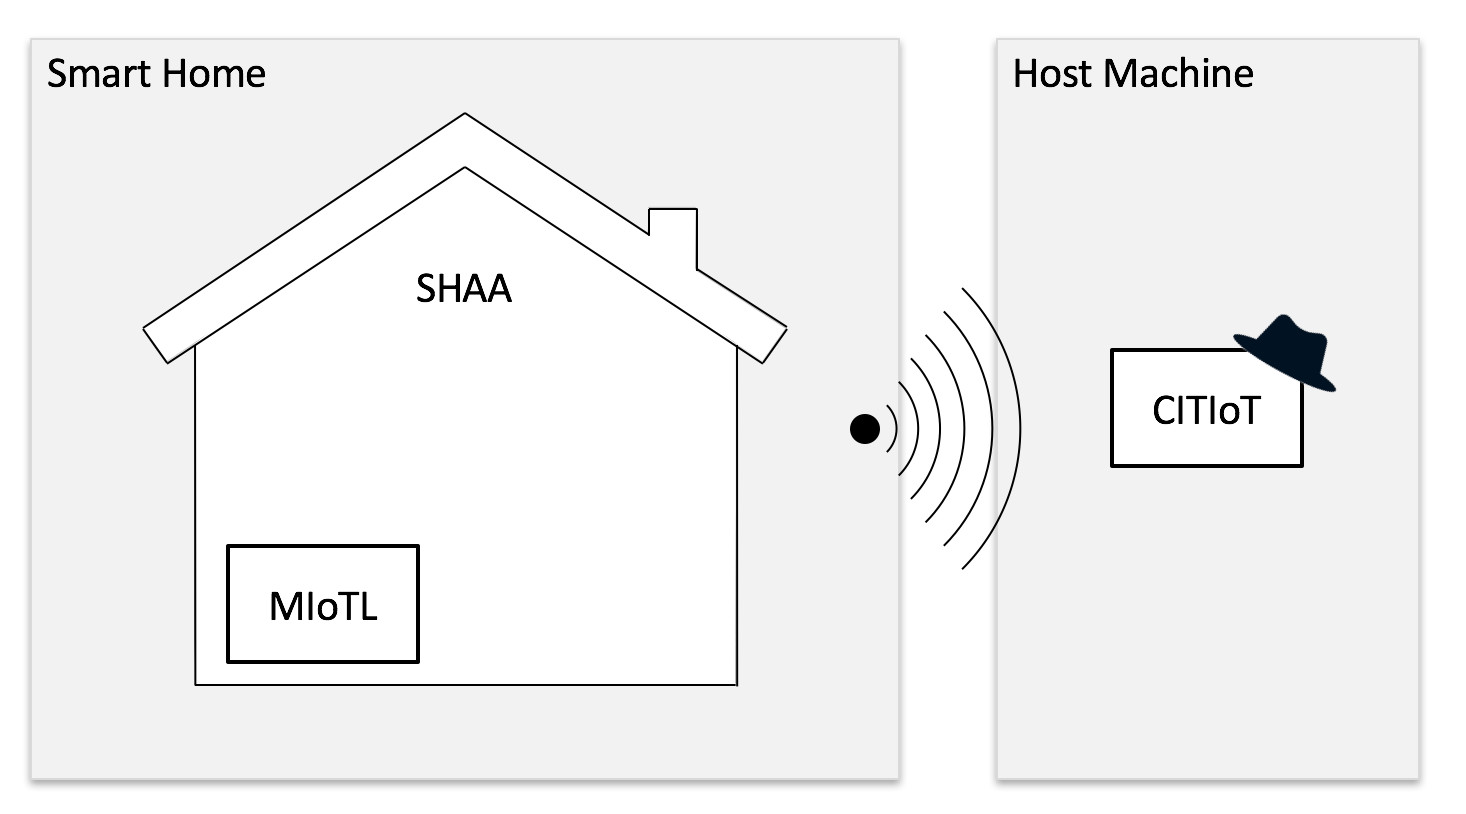
\includegraphics[width=4in]{systemDiagram}}
			\caption{Overall system diagram}
			\label{fig:SystemDiagram}
		\end{center}
		\vspace{-0.2 in}
	\end{figure}
}

\newcommand{\figShaaDiagram}{
	\begin{figure*}[h!]
		\begin{center}
			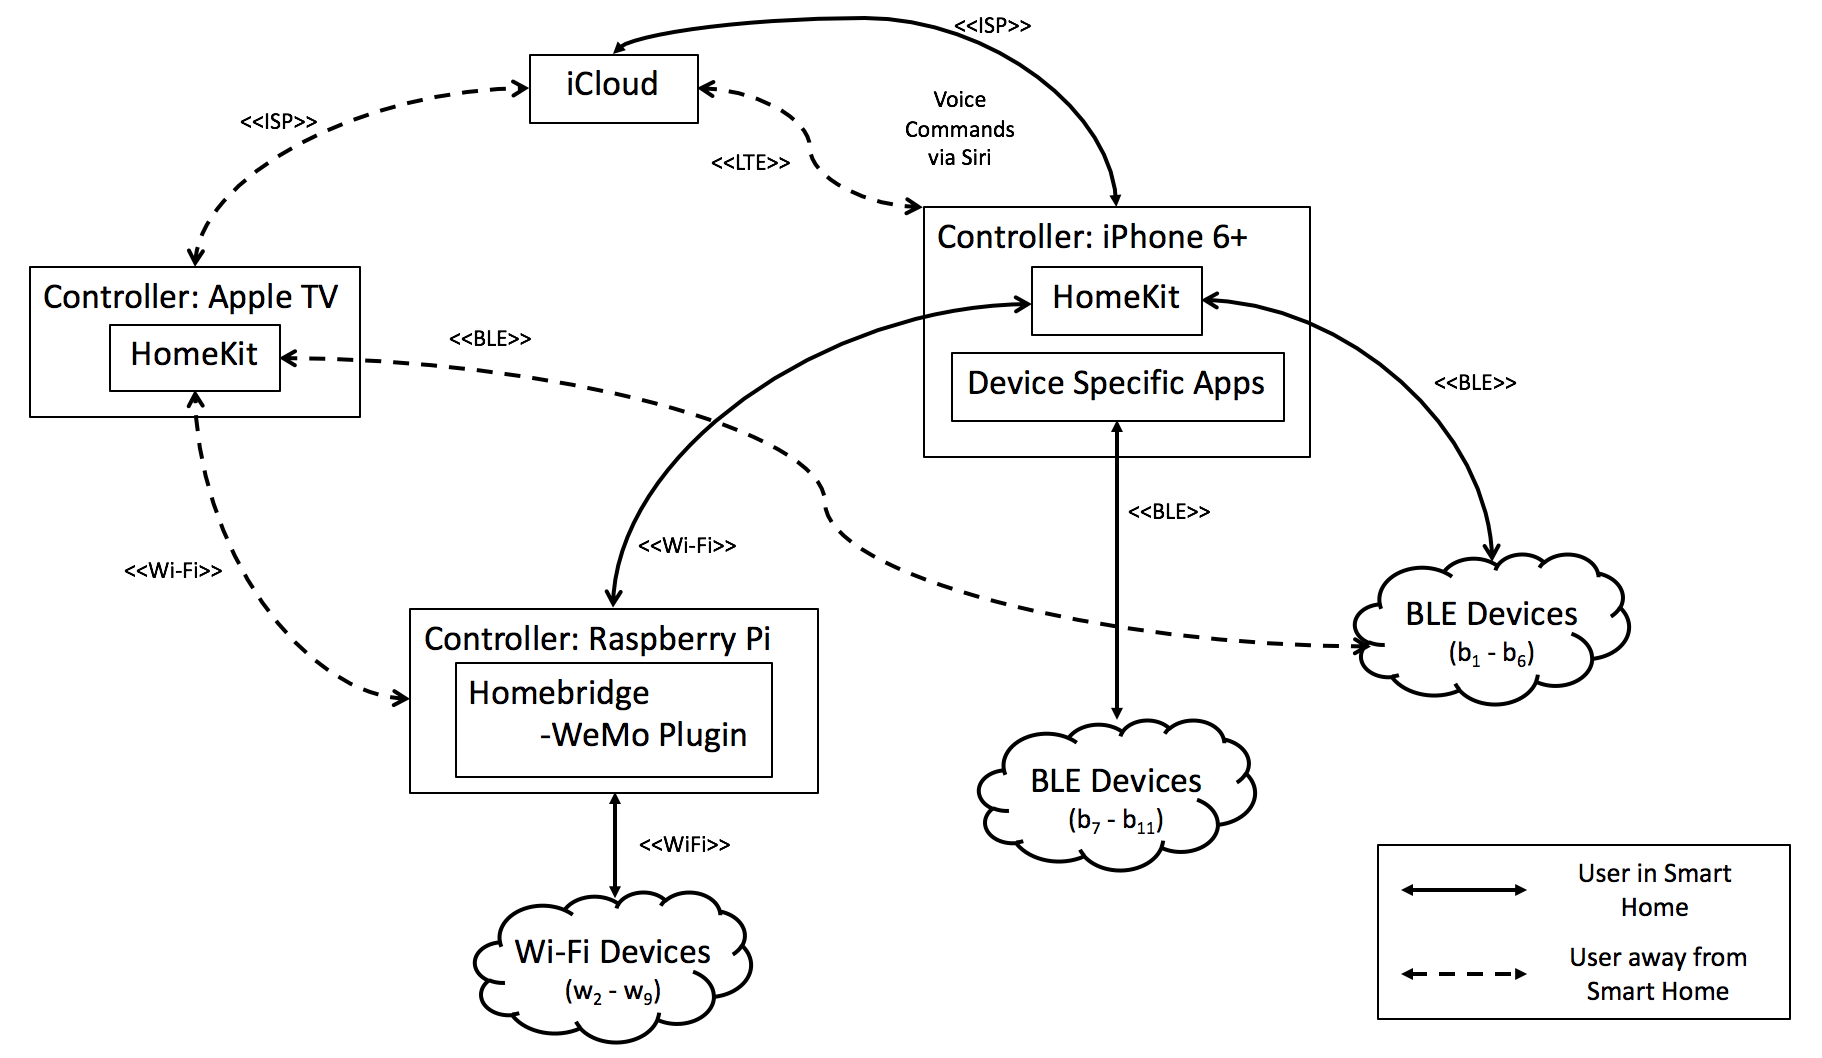
\includegraphics[width=\linewidth]{shaaDiagram}
			\caption{Diagram of SHAA components}
			\label{fig:ShaaDiagram}
		\end{center}
		\vspace{-0.2 in}
	\end{figure*}
}

\newcommand{\figCitiotDiagram}{
	\begin{figure*}[h!]
		\begin{center}
			\makebox[\textwidth][c]{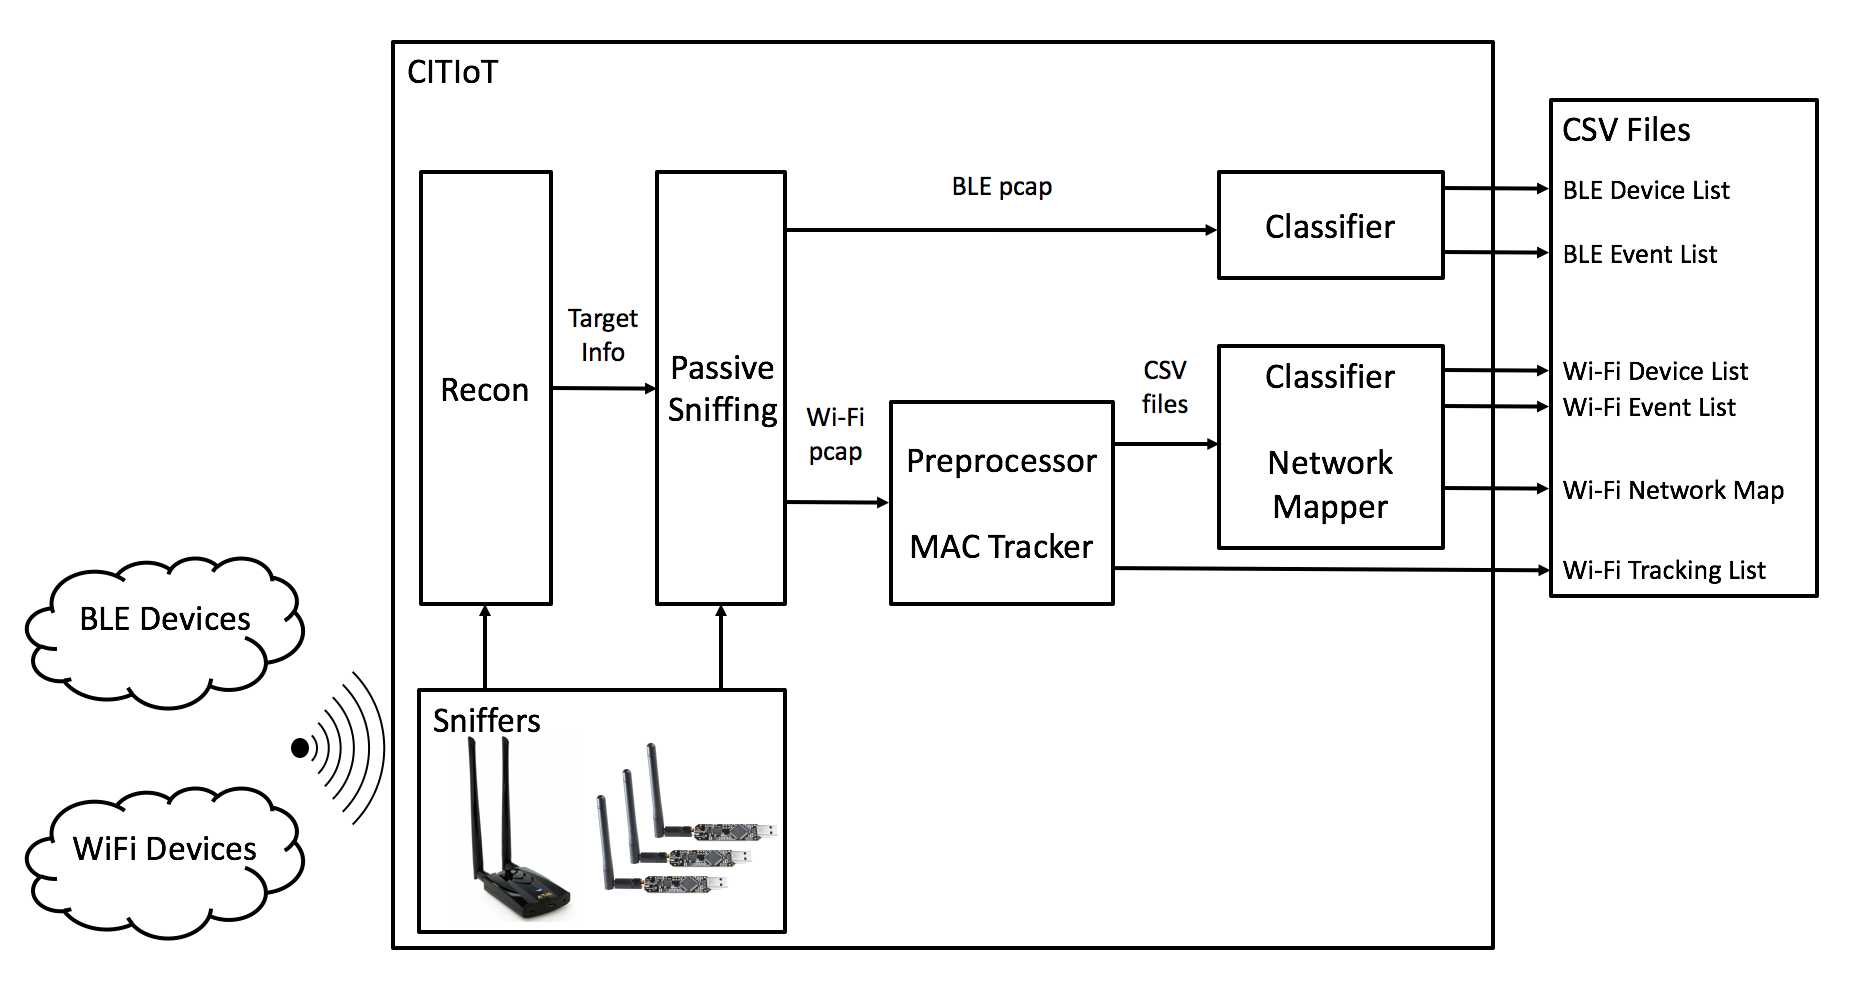
\includegraphics[width=\linewidth]{citiotDiagram}}
			\caption{Diagram of CITIoT tool components and interactions}
			\label{fig:CitiotDiagram}
		\end{center}
		\vspace{-0.2 in}
	\end{figure*}
}

\newcommand{\figReconScan}{
	\begin{figure*}[h!]
		\begin{center}
			\makebox[\textwidth][c]{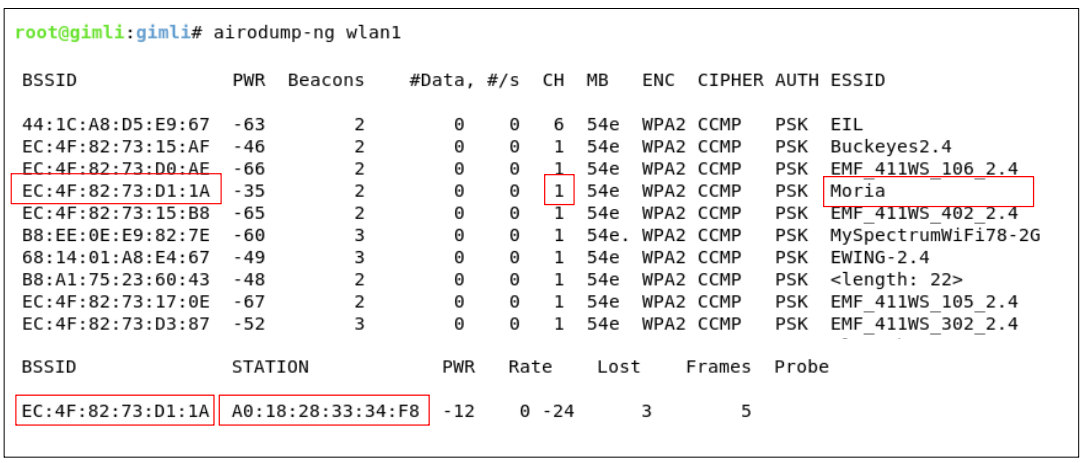
\includegraphics[width=\linewidth]{reconScan}}
			\caption{Command and results to accomplish a scan of Wi-Fi devices and associated \ac{AP}s}
			\label{fig:ReconScan}
		\end{center}
		\vspace{-0.2 in}
	\end{figure*}
}

\newcommand{\figScanDevices}{
	\begin{figure}[H]
		\begin{center}
			\makebox[\textwidth][c]{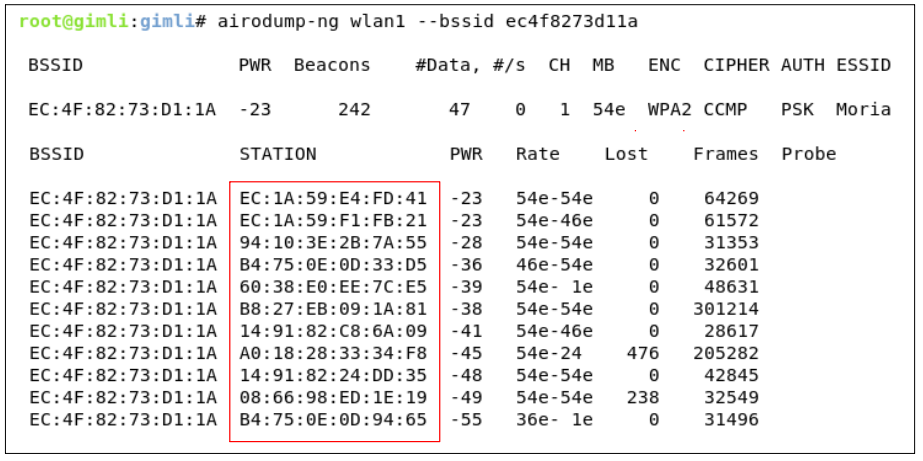
\includegraphics[width=\linewidth]{scanDevices}}
			\caption{Command and results to scan for devices connected to the target \ac{AP}}
			\label{fig:ScanDevices}
		\end{center}
		\vspace{-0.2 in}
	\end{figure}
}

\newcommand{\figOuiLookup}{
	\begin{figure}[H]
		\begin{center}
			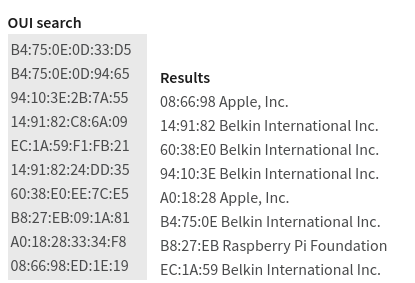
\includegraphics[width=3in]{ouiLookup}
			\caption{Wi-Fi MAC OUI search and results}
			\label{fig:OuiLookup}
		\end{center}
		\vspace{-0.2 in}
	\end{figure}
}

\newcommand{\figBleDeviceScan}{
	\begin{figure}[H]
		\begin{center}
			\makebox[\textwidth][c]{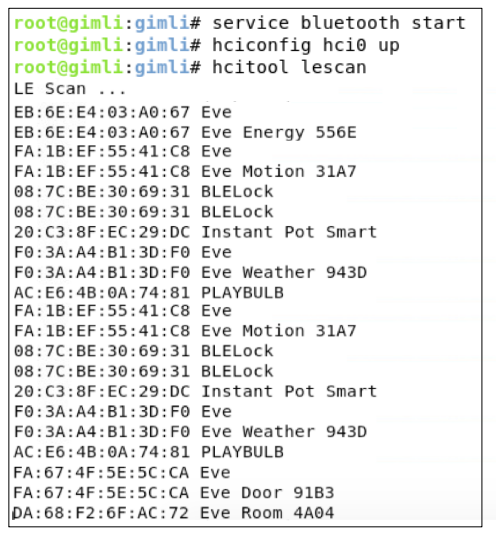
\includegraphics[width=3.5in]{bleDeviceScan}}
			\caption{Command and results to scan for \ac{BLE} devices within the smart home}
			\label{fig:BleDeviceScan}
		\end{center}
		\vspace{-0.2 in}
	\end{figure}
}

\newcommand{\figMonitorMode}{
	\begin{figure}[H]
		\begin{center}
			\makebox[\textwidth][c]{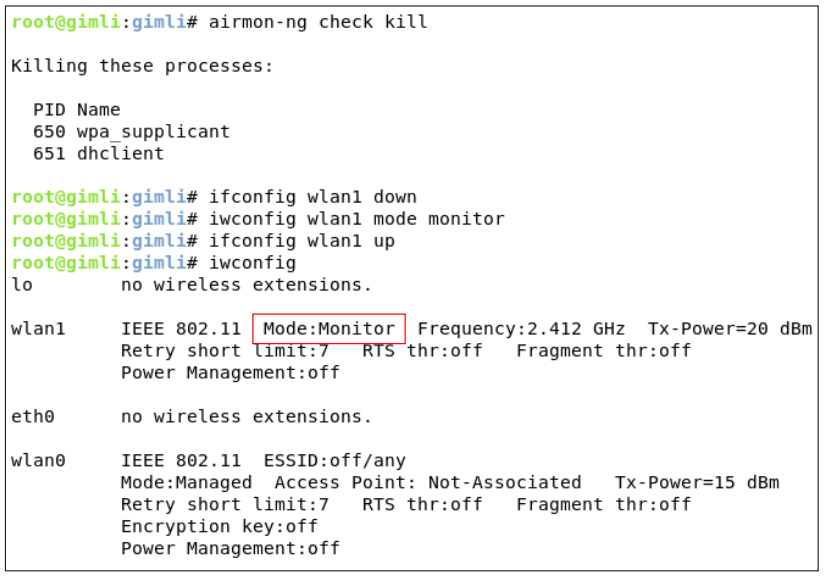
\includegraphics[width=\linewidth]{monitorMode}}
			\caption{Commands used to set Wi-Fi interface to monitor mode}
			\label{fig:MonitorMode}
		\end{center}
		\vspace{-0.2 in}
	\end{figure}
}

\newcommand{\figWifiCaptCmd}{
	\begin{figure}[H]
		\begin{center}
			\makebox[\textwidth][c]{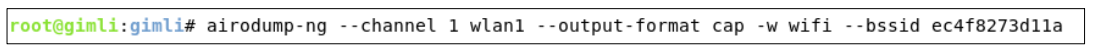
\includegraphics[height=.75cm]{wifiCaptCmd}}
			\caption{Command and options used to capture Wi-Fi traffic}
			\label{fig:WifiCaptCmd}
		\end{center}
		\vspace{-0.2 in}
	\end{figure}
}

\newcommand{\figBleCaptCmd}{
	\begin{figure}[H]
		\begin{center}
			\makebox[\textwidth][c]{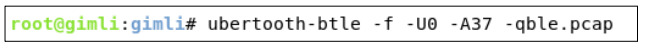
\includegraphics[height=.75cm]{bleCaptCmd}}
			\caption{Example command and options used to capture \ac{BLE} traffic}
			\label{fig:BleCaptCmd}
		\end{center}
		\vspace{-0.2 in}
	\end{figure}
}

\newcommand{\figCorruptTimePacket}{
	\begin{figure}[H]
		\begin{center}
			\makebox[\textwidth][c]{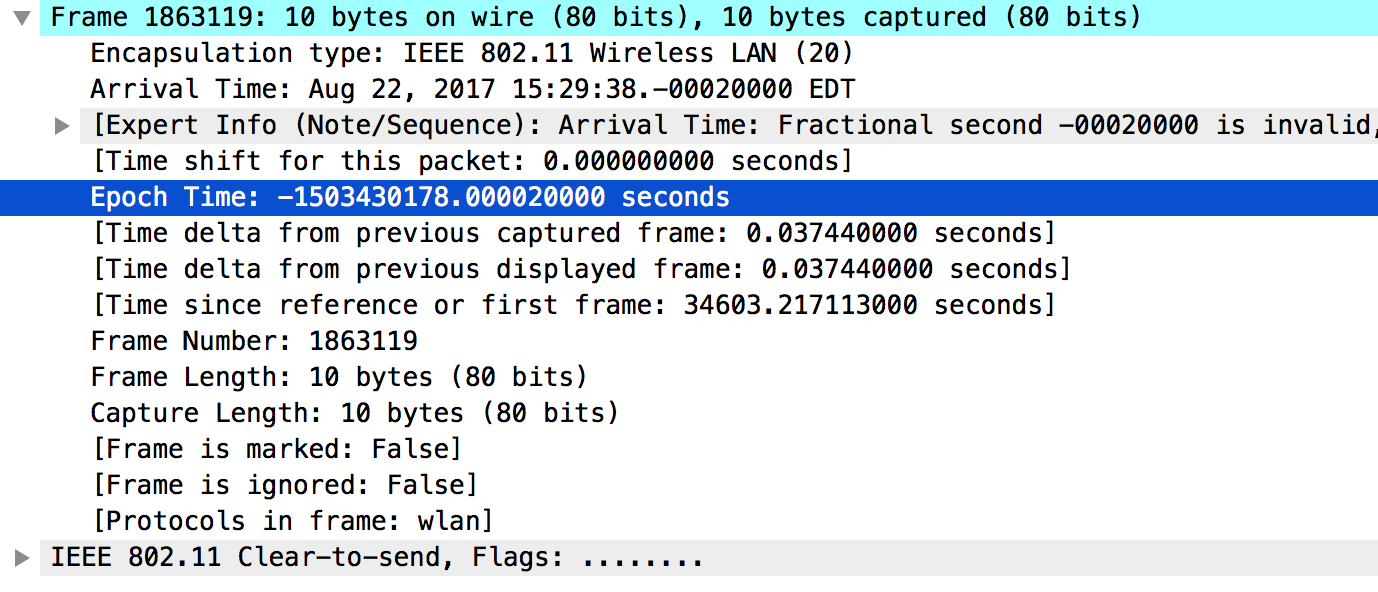
\includegraphics[width=\linewidth]{corruptTimePacket}}
			\caption{Encrypted packet used in \ac{MAC} tracker showing corrupted timestamp}
			\label{fig:CorruptTimePacket}
		\end{center}
		\vspace{-0.2 in}
	\end{figure}
}

\newcommand{\figWrongFrameNumber}{
	\begin{figure}[H]
		\begin{center}
			\makebox[\textwidth][c]{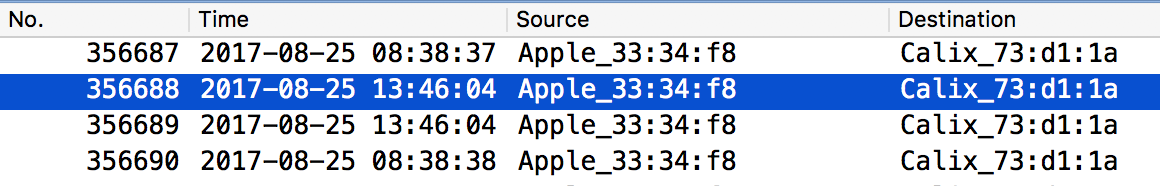
\includegraphics[width=\linewidth]{wrongFrameNumber}}
			\caption{Encrypted packets used in \ac{MAC} tracker showing sequential frame numbers but wrong times}
			\label{fig:WrongFrameNumber}
		\end{center}
		\vspace{-0.2 in}
	\end{figure}
}

\newcommand{\figTrainingToDevice}{
	\begin{figure}[H]
		\centering
		\begin{subfigure}{.485\textwidth}
			\centering
			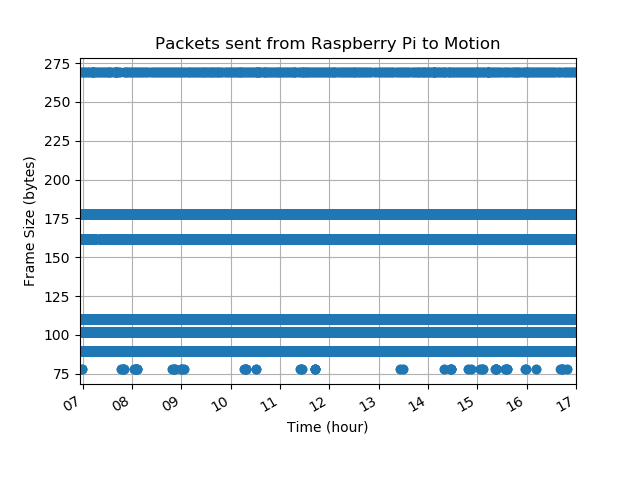
\includegraphics[width=\linewidth]{trngToMotion}
			\caption{}
		\end{subfigure}%
		\begin{subfigure}{.485\textwidth}
			\centering
			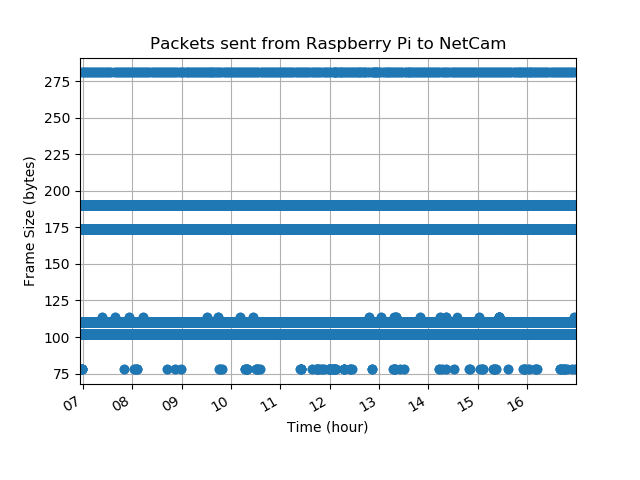
\includegraphics[width=\linewidth]{trngToNetcam}
			\caption{}
		\end{subfigure}
		\begin{subfigure}{.485\textwidth}
			\centering
			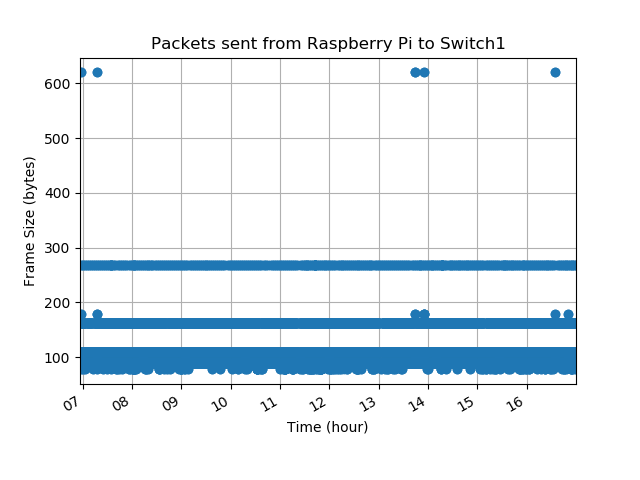
\includegraphics[width=\linewidth]{trngToSwitch1}
			\caption{}
		\end{subfigure}%
		\begin{subfigure}{.485\textwidth}
			\centering
			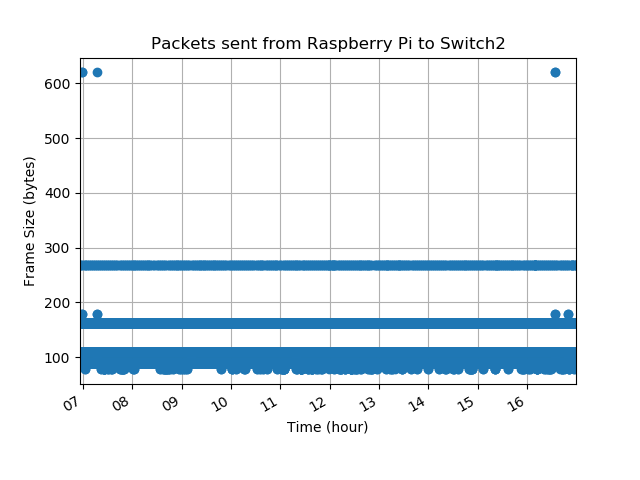
\includegraphics[width=\linewidth]{trngToSwitch2}
			\caption{}
		\end{subfigure}
		\begin{subfigure}{.485\textwidth}
			\centering
			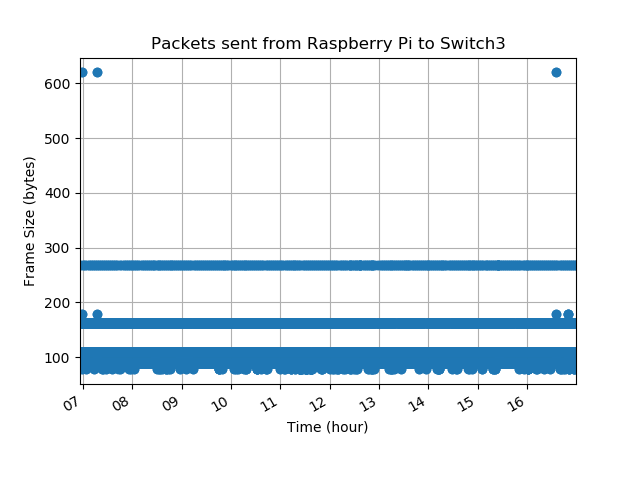
\includegraphics[width=\linewidth]{trngToSwitch3}
			\caption{}
		\end{subfigure}%
		\begin{subfigure}{.485\textwidth}
			\centering
			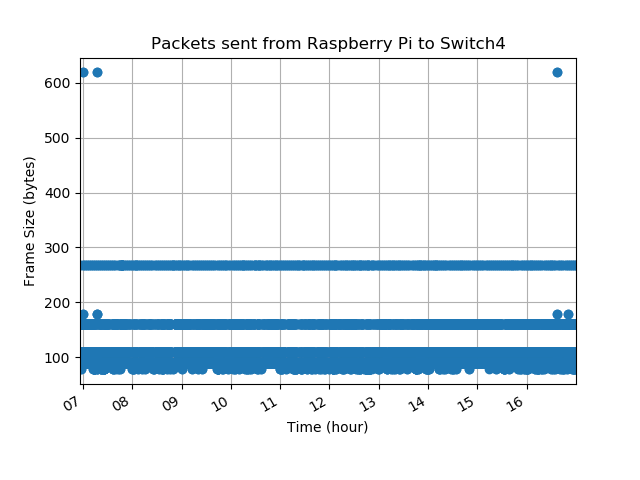
\includegraphics[width=\linewidth]{trngToSwitch4}
			\caption{}
		\end{subfigure}
		\begin{subfigure}{.485\textwidth}
			\centering
			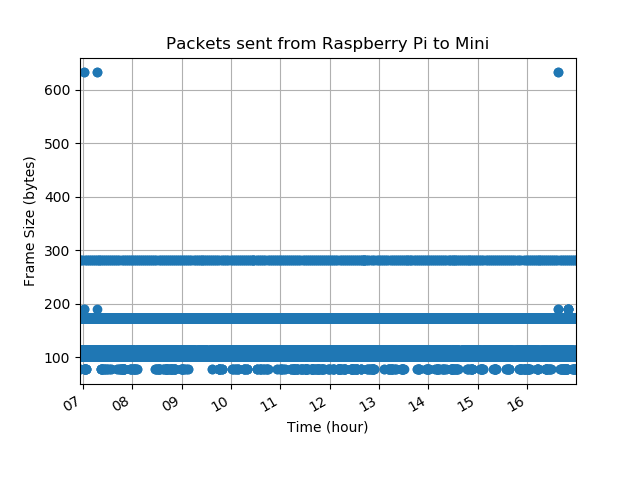
\includegraphics[width=\linewidth]{trngToMini}
			\caption{}
		\end{subfigure}%
		\begin{subfigure}{.485\textwidth}
			\centering
			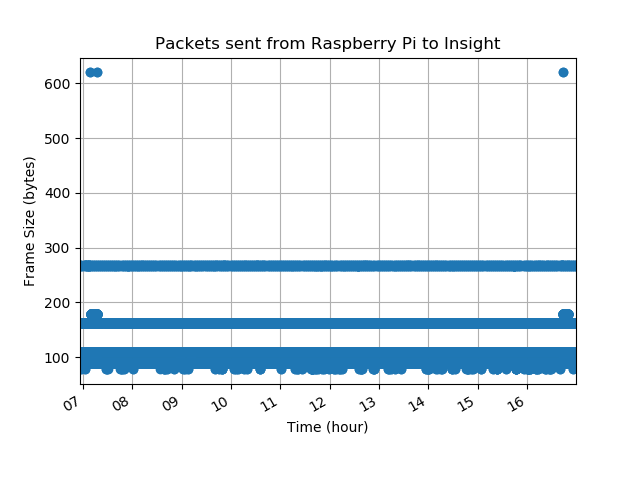
\includegraphics[width=\linewidth]{trngToInsight}
			\caption{}
		\end{subfigure}
		\caption{Training plots of packets sent from raspberry pi to device}
		\label{fig:TrainingToDevice}
	\end{figure}
}

\newcommand{\figTrainingFromDevice}{
	\begin{figure}[H]
		\centering
		\begin{subfigure}{.485\textwidth}
			\centering
			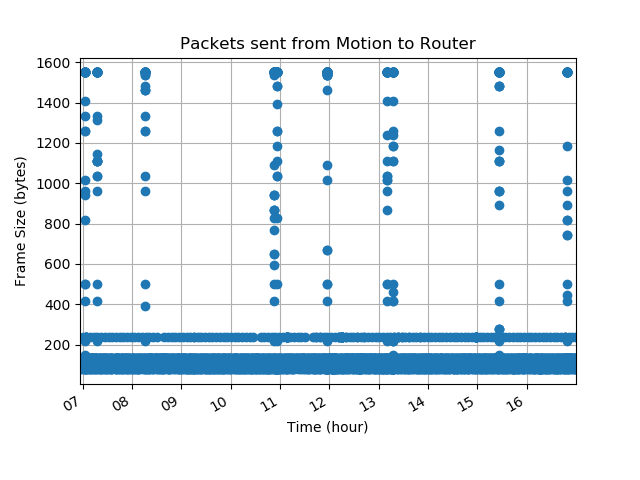
\includegraphics[width=\linewidth]{trngFromMotion}
			\caption{}
		\end{subfigure}%
		\begin{subfigure}{.485\textwidth}
			\centering
			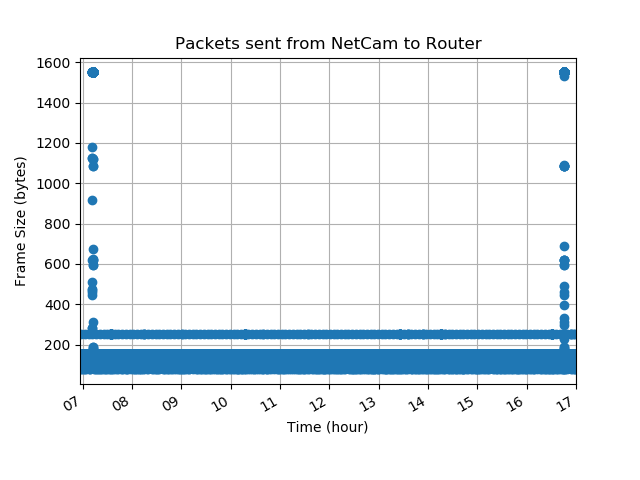
\includegraphics[width=\linewidth]{trngFromNetcam}
			\caption{}
		\end{subfigure}
		\begin{subfigure}{.485\textwidth}
			\centering
			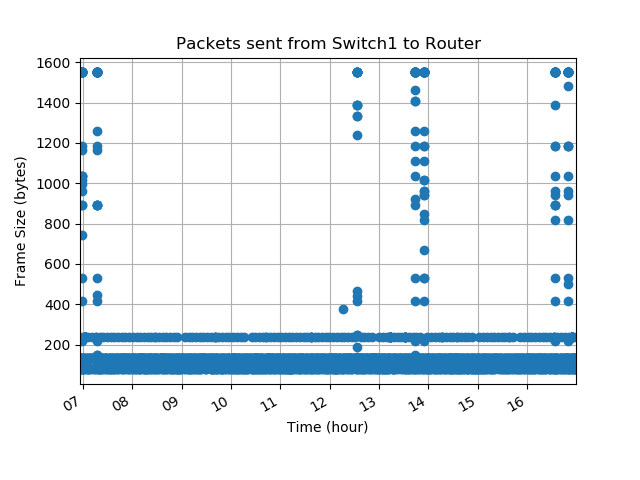
\includegraphics[width=\linewidth]{trngFromSwitch1}
			\caption{}
		\end{subfigure}%
		\begin{subfigure}{.485\textwidth}
			\centering
			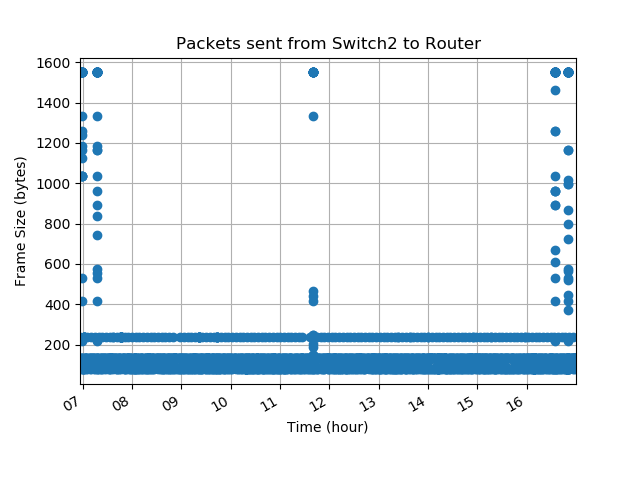
\includegraphics[width=\linewidth]{trngFromSwitch2}
			\caption{}
		\end{subfigure}
		\begin{subfigure}{.485\textwidth}
			\centering
			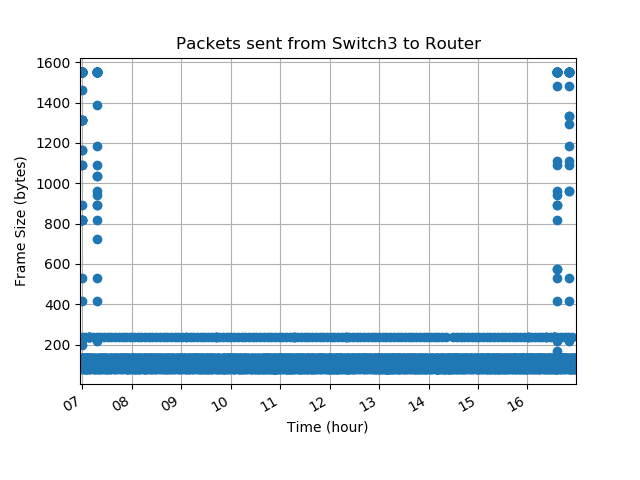
\includegraphics[width=\linewidth]{trngFromSwitch3}
			\caption{}
		\end{subfigure}%
		\begin{subfigure}{.485\textwidth}
			\centering
			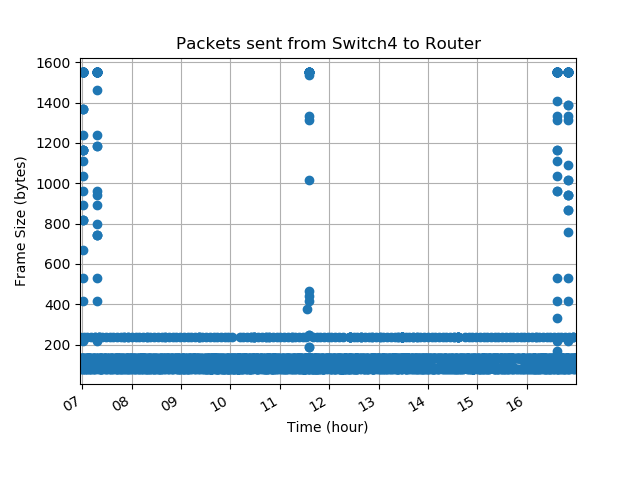
\includegraphics[width=\linewidth]{trngFromSwitch4}
			\caption{}
		\end{subfigure}
		\begin{subfigure}{.485\textwidth}
			\centering
			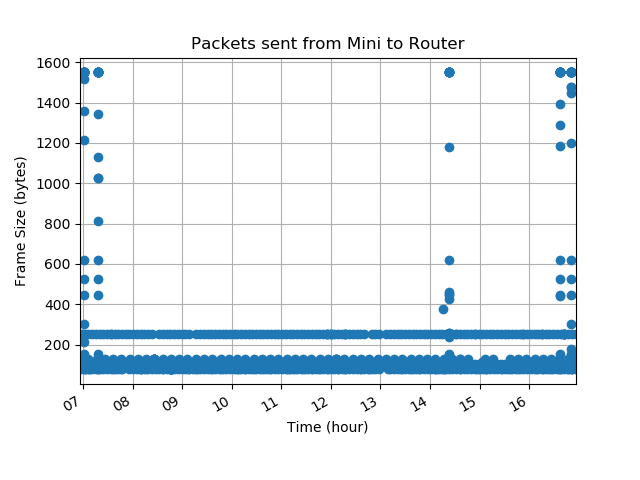
\includegraphics[width=\linewidth]{trngFromMini}
			\caption{}
		\end{subfigure}%
		\begin{subfigure}{.485\textwidth}
			\centering
			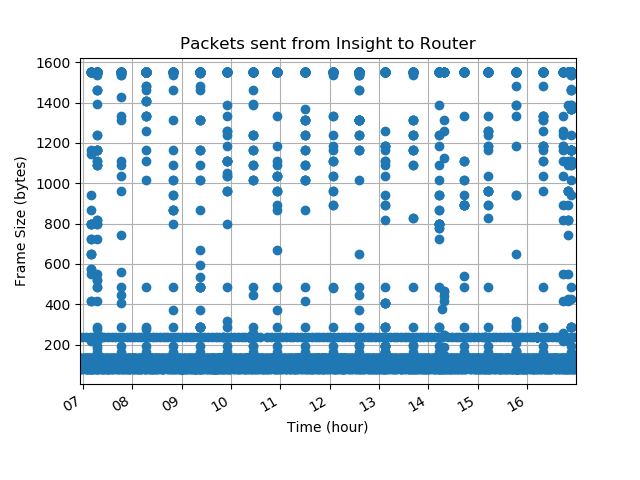
\includegraphics[width=\linewidth]{trngFromInsight}
			\caption{}
		\end{subfigure}
		\caption{Training plots of packets sent from device to the router}
		\label{fig:TrainingFromDevice}
	\end{figure}
}

\newcommand{\figClassificationToNetcam}{
	\begin{figure}[H]
		\begin{center}
			\makebox[\textwidth][c]{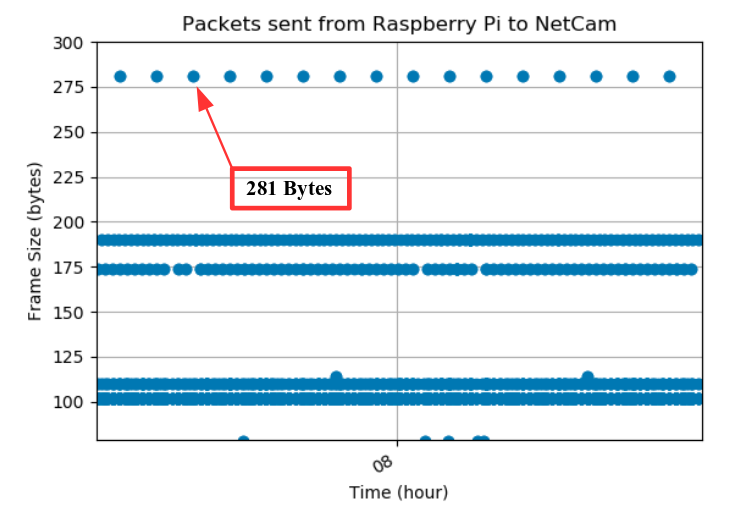
\includegraphics[width=5in]{classificationToNetcam}}
			\caption{Figure~\ref{fig:TrainingToDevice}(b) zoomed in on unique packet traffic used to classify camera devices}
			\label{fig:ClassificationToNetcam}
		\end{center}
		\vspace{-0.2 in}
	\end{figure}
}

\newcommand{\figClassificationToMotion}{
	\begin{figure}[H]
		\begin{center}
			\makebox[\textwidth][c]{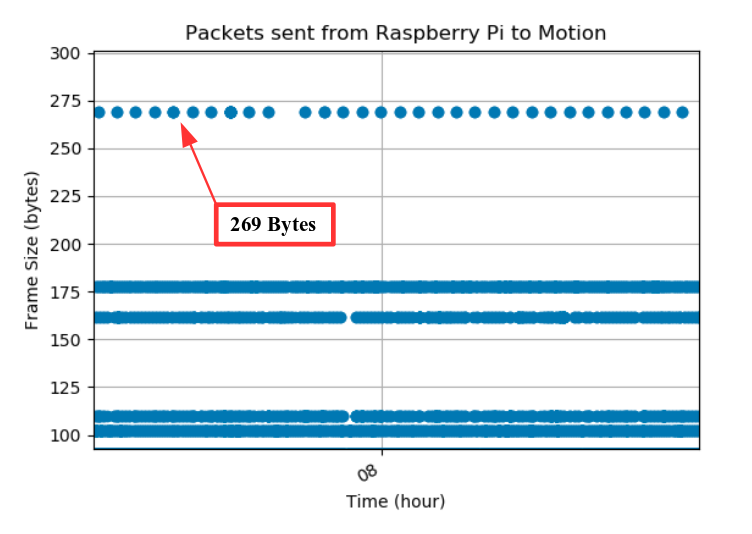
\includegraphics[width=5in]{classificationToMotion}}
			\caption{Figure~\ref{fig:TrainingToDevice}(a) zoomed in on unique packet traffic used to classify motion devices}
			\label{fig:ClassificationToMotion}
		\end{center}
		\vspace{-0.2 in}
	\end{figure}
}

\newcommand{\figClassificationToSwitch}{
	\begin{figure}[H]
		\begin{center}
			\makebox[\textwidth][c]{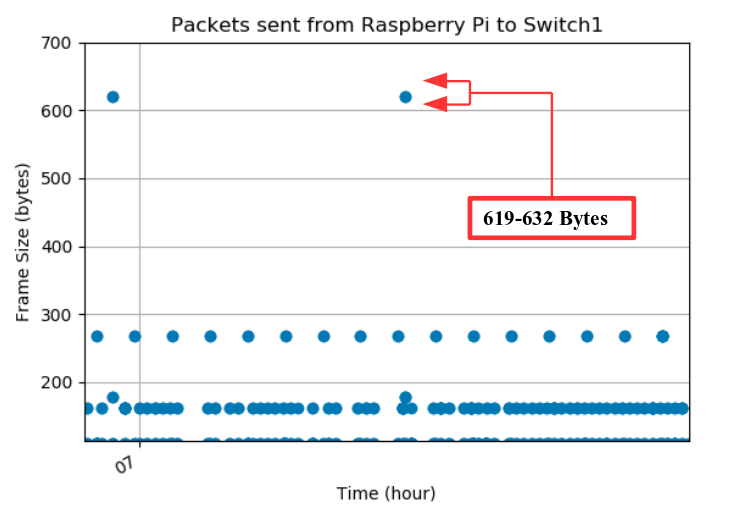
\includegraphics[width=5in]{classificationToSwitch}}
			\caption{Figure~\ref{fig:TrainingToDevice}(c) zoomed in on unique packet traffic used to classify outlet devices}
			\label{fig:ClassificationToSwitch}
		\end{center}
		\vspace{-0.2 in}
	\end{figure}
}

\newcommand{\figDeviceClassification}{
	\begin{figure}[H]
		\begin{center}
			\makebox[\textwidth][c]{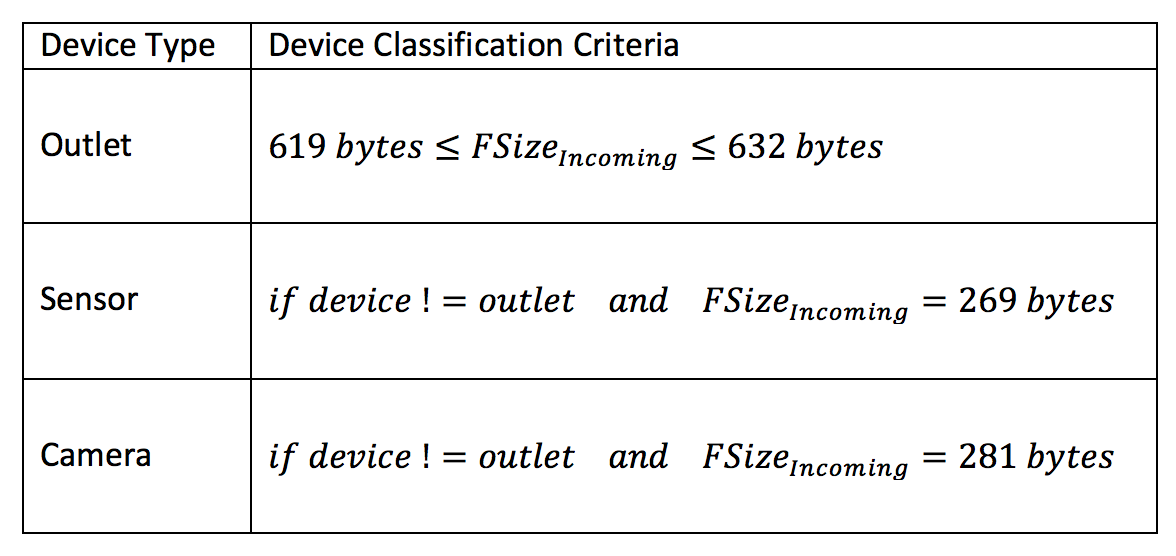
\includegraphics[height=2in]{deviceClassification}}
			\caption{Criteria used to classify devices}
			\label{fig:DeviceClassification}
		\end{center}
		\vspace{-0.2 in}
	\end{figure}
}

\newcommand{\figIdentificationToMini}{
	\begin{figure}[H]
		\begin{center}
			\makebox[\textwidth][c]{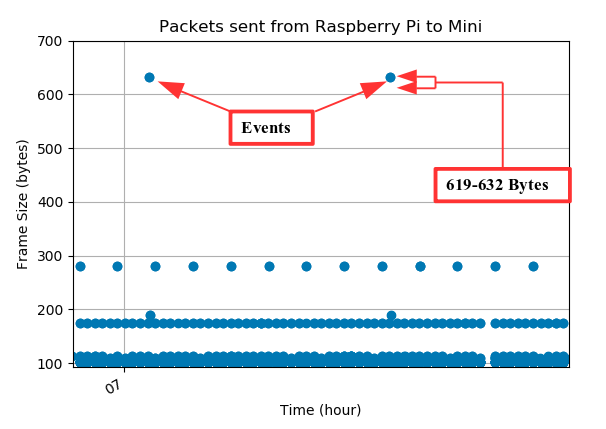
\includegraphics[width=5in]{identificationToMini}}
			\caption{Figure~\ref{fig:TrainingToDevice}(g) zoomed in on unique packet traffic used to identify outlet events}
			\label{fig:IdentificationToMini}
		\end{center}
		\vspace{-0.2 in}
	\end{figure}
}

\newcommand{\figIdentificationFromNetcam}{
	\begin{figure}[H]
		\begin{center}
			\makebox[\textwidth][c]{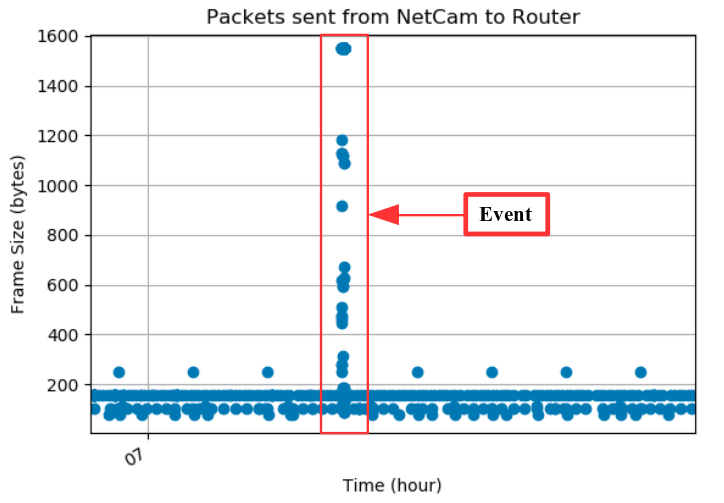
\includegraphics[width=5in]{identificationFromNetcam}}
			\caption{Figure~\ref{fig:TrainingFromDevice}(b) zoomed in on unique packet traffic used to identify camera events}
			\label{fig:IdentificationFromNetcam}
		\end{center}
		\vspace{-0.2 in}
	\end{figure}
}

\newcommand{\figIdentificationFromNetcamCum}{
	\begin{figure}[H]
		\begin{center}
			\makebox[\textwidth][c]{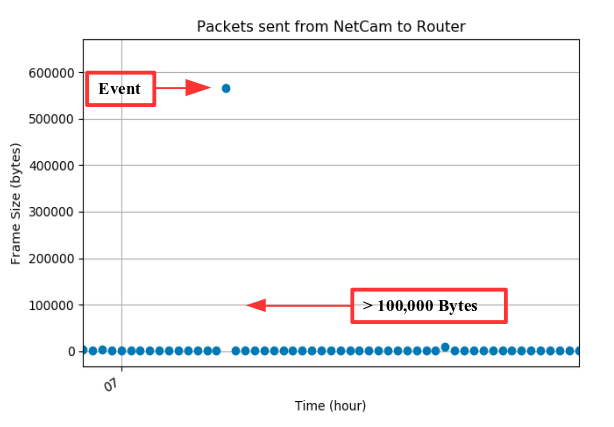
\includegraphics[width=5in]{identificationFromNetcamCum}}
			\caption{Figure~\ref{fig:TrainingFromDevice}(b) with one minute cumulative frame size zoomed in on unique packet traffic used to identify camera events}
			\label{fig:IdentificationFromNetcamCum}
		\end{center}
		\vspace{-0.2 in}
	\end{figure}
}

\newcommand{\figIdentificationFromMotion}{
	\begin{figure}[H]
		\begin{center}
			\makebox[\textwidth][c]{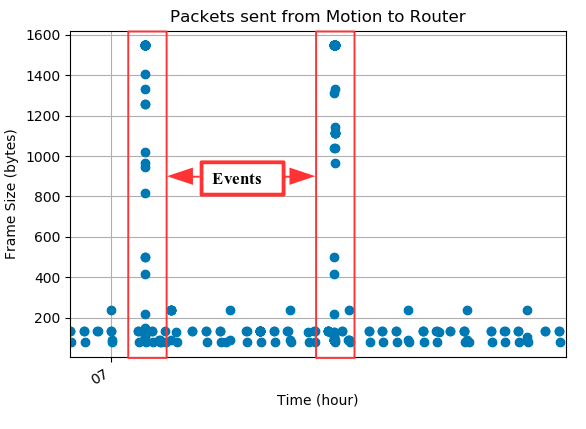
\includegraphics[width=5in]{identificationFromMotion}}
			\caption{Figure~\ref{fig:TrainingFromDevice}(a) zoomed in on unique packet traffic used to identify motion events}
			\label{fig:IdentificationFromMotion}
		\end{center}
		\vspace{-0.2 in}
	\end{figure}
}

\newcommand{\figIdentificationFromMotionCum}{
	\begin{figure}[H]
		\begin{center}
			\makebox[\textwidth][c]{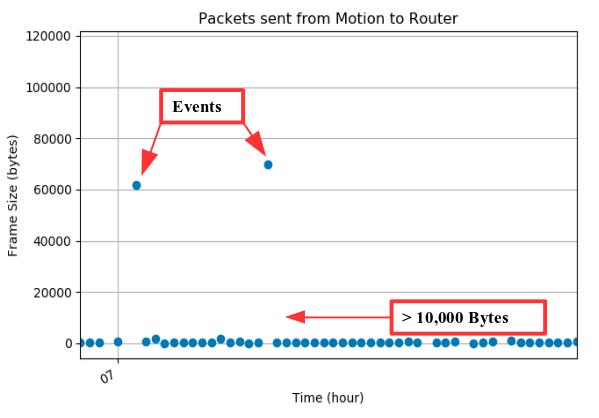
\includegraphics[width=5in]{identificationFromMotionCum}}
			\caption{Figure~\ref{fig:TrainingFromDevice}(a) with one minute cumulative frame size zoomed in on unique packet traffic used to identify motion events}
			\label{fig:IdentificationFromMotionCum}
		\end{center}
		\vspace{-0.2 in}
	\end{figure}
}

\newcommand{\figEventIdentification}{
	\begin{figure}[H]
		\begin{center}
			\makebox[\textwidth][c]{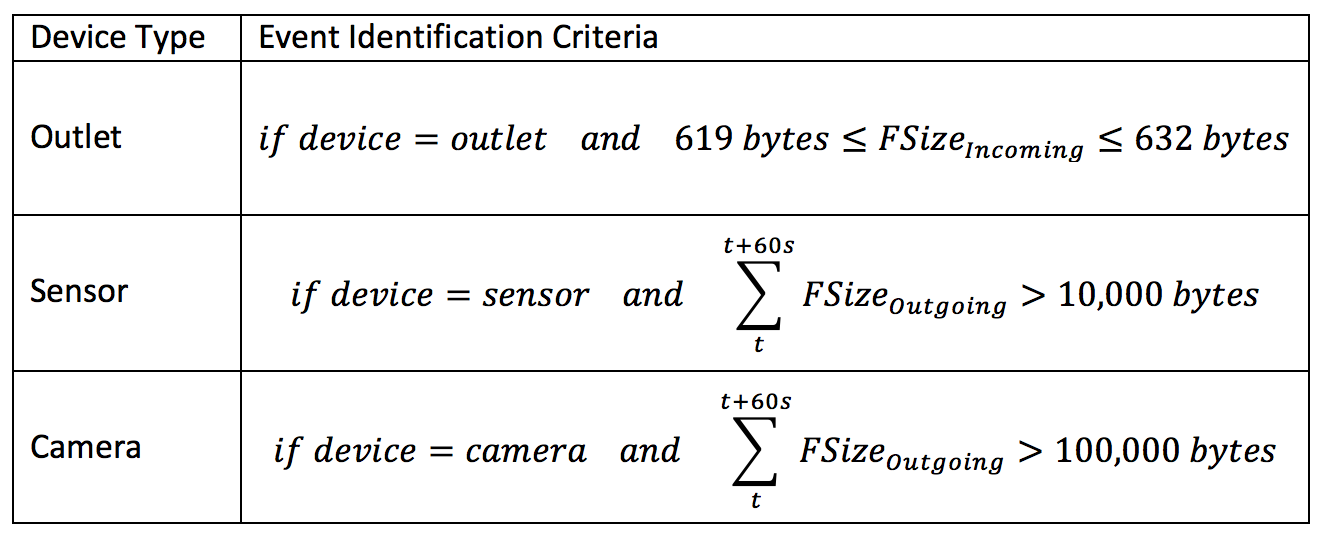
\includegraphics[height=2in]{eventIdentification}}
			\caption{Criteria used to identify events}
			\label{fig:EventIdentification}
		\end{center}
		\vspace{-0.2 in}
	\end{figure}
}

\newcommand{\figSubscribePacket}{
	\begin{figure}[H]
		\begin{center}
			\makebox[\textwidth][c]{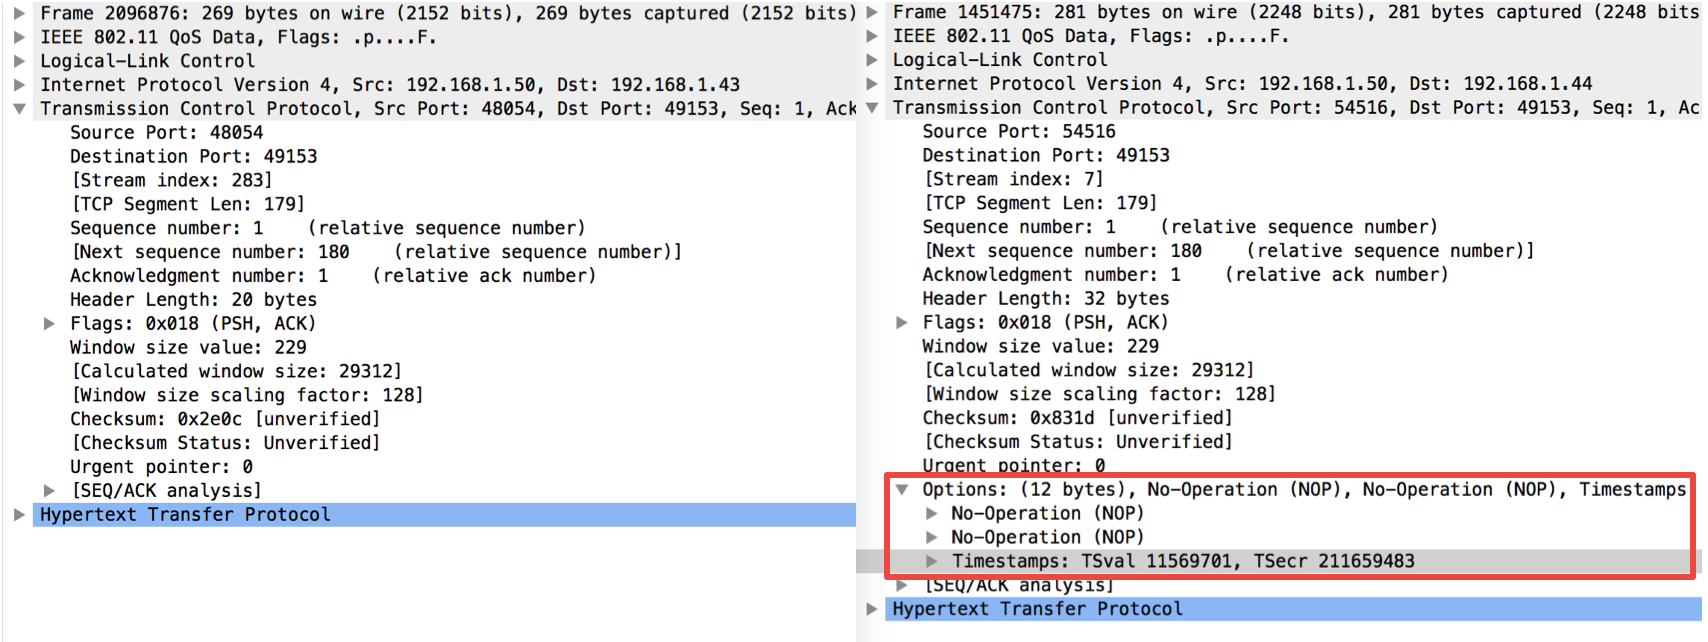
\includegraphics[width=\linewidth]{subscribePacket}}
			\caption{Decrypted \texttt{SUBSCRIBE} packets from Raspberry Pi to the NetCam and Motion devices depicting difference in frame length}
			\label{fig:SubscribePacket}
		\end{center}
		\vspace{-0.2 in}
	\end{figure}
}

\newcommand{\figPostPacket}{
	\begin{figure}[H]
		\begin{center}
			\makebox[\textwidth][c]{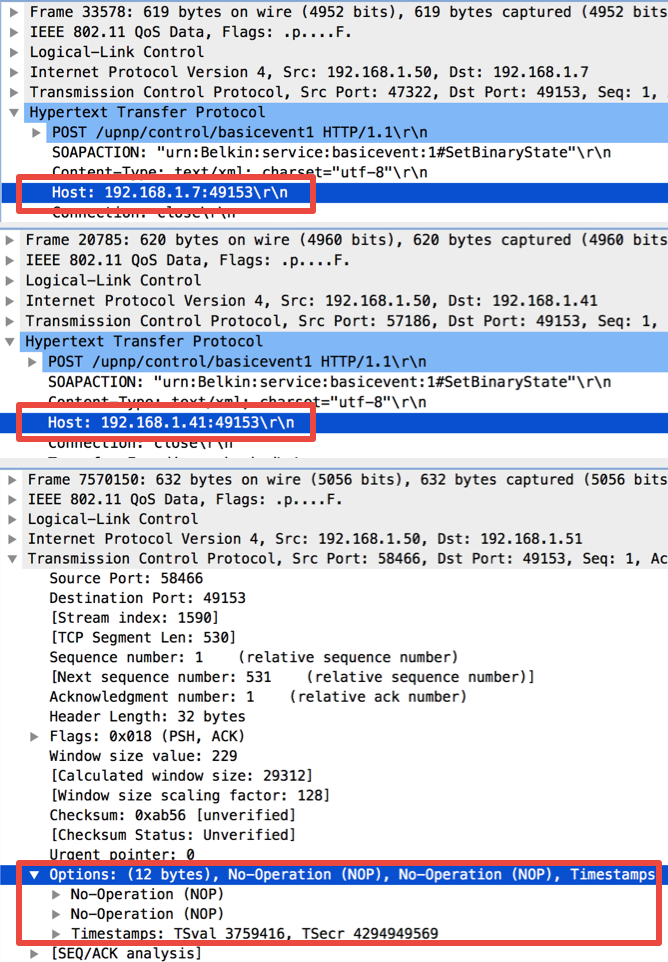
\includegraphics[width=.975\linewidth]{postPacket}}
			\caption{Decrypted \texttt{POST} packets from Raspberry Pi to the Switch4, Switch2, and Mini depicting differences in frame length}
			\label{fig:PostPacket}
		\end{center}
		\vspace{-0.2 in}
	\end{figure}
}

\newcommand{\figNetworkMap}{
	\begin{figure}[H]
		\begin{center}
			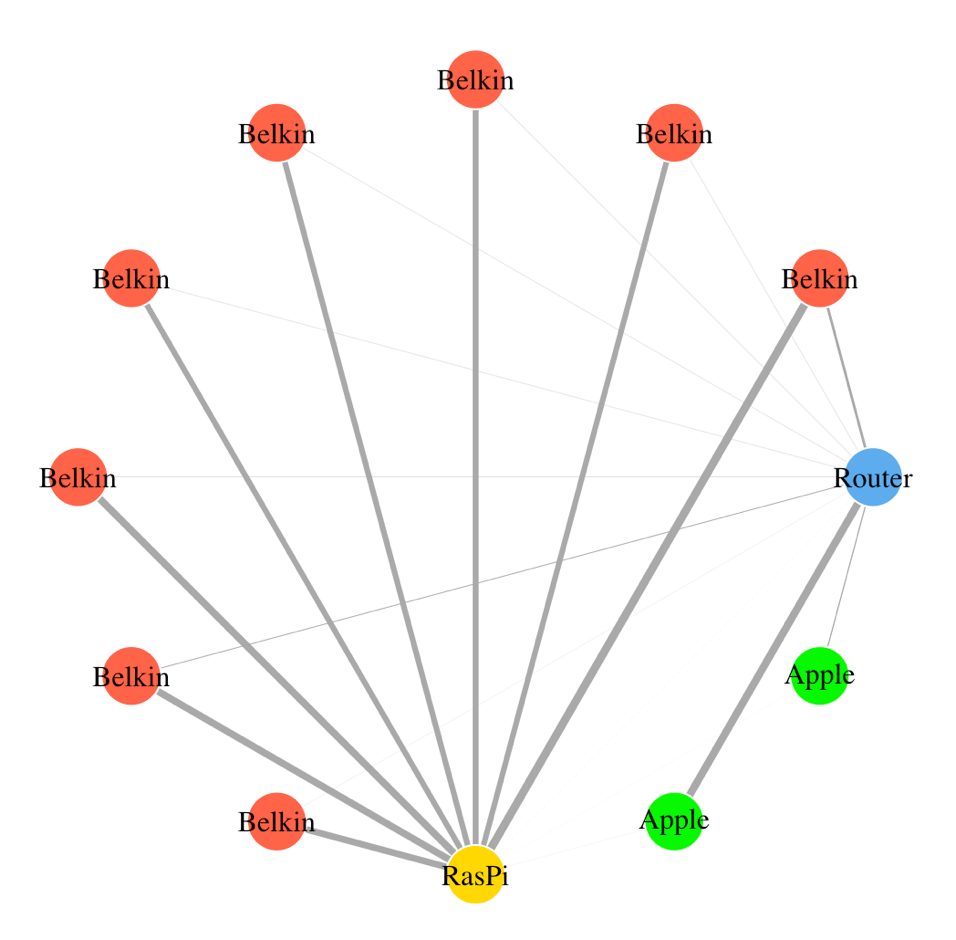
\includegraphics[width=5in]{networkMap}
			\caption{Network mapping of smart home architecture}
			\label{fig:NetworkMap}
		\end{center}
		\vspace{-0.2 in}
	\end{figure}
}

\newcommand{\figMiotlDiagram}{
	\begin{figure*}[h!]
		\begin{center}
			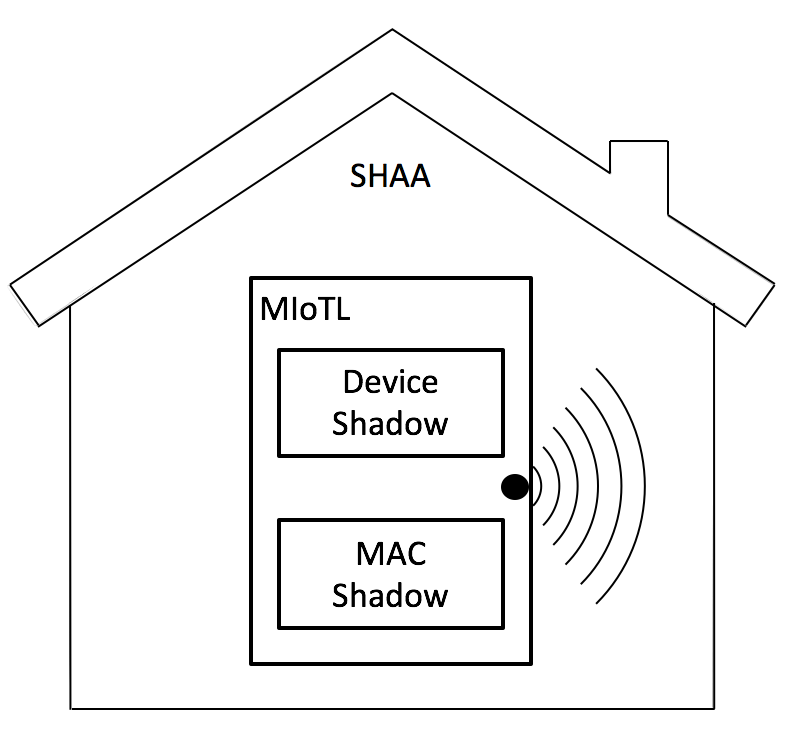
\includegraphics[width=3in]{miotlDiagram}
			\caption{Diagram of MIoTL tool components}
			\label{fig:MiotlDiagram}
		\end{center}
		\vspace{-0.2 in}
	\end{figure*}
}

\newcommand{\figSutCutDiagram}{
	\begin{figure*}[h!]
		\begin{center}
			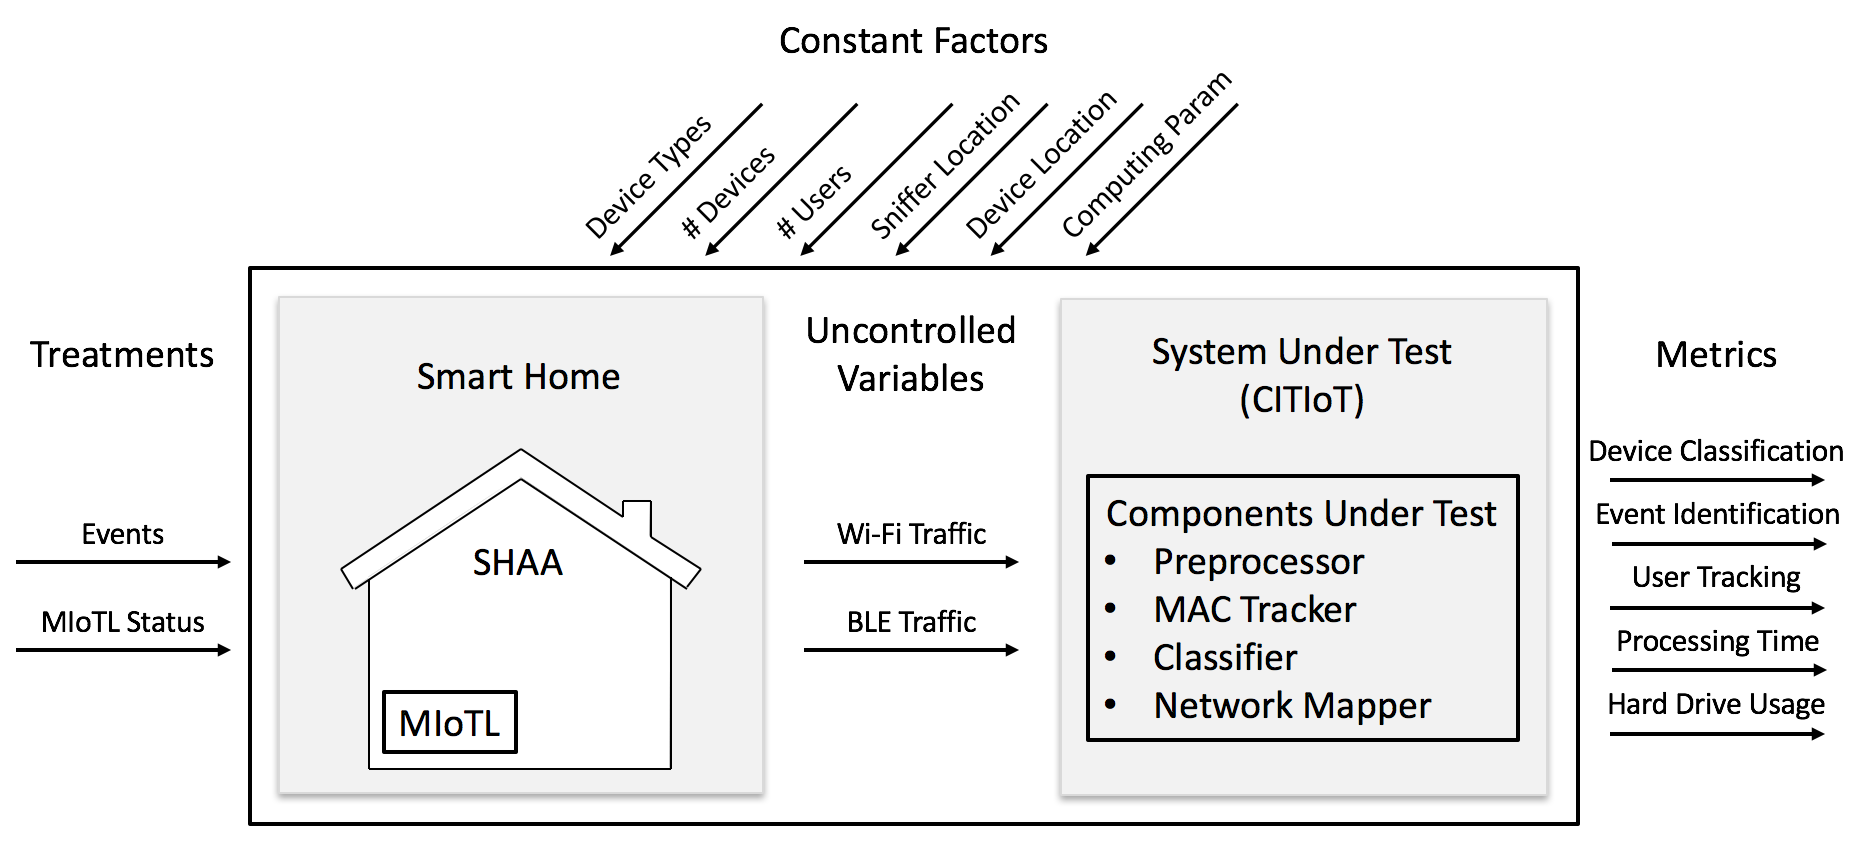
\includegraphics[width=\linewidth]{sutCutDiagram}
			\caption{System Under Test (SUT) and Component Under Test (CUT) diagram}
			\label{fig:SutCutDiagram}
		\end{center}
		\vspace{-0.2 in}
	\end{figure*}
}

\newcommand{\figShaaExperimentDiagram}{
	\begin{figure*}[h!]
		\begin{center}
			\includegraphics[width=\linewidth]{shaaExperimentDiagram}
			\caption{Approximate layout of devices within \ac{SHAA} for experimentation (not to scale)}
			\label{fig:ShaaExperimentDiagram}
		\end{center}
		\vspace{-0.2 in}
	\end{figure*}
}

\newcommand{\figSnifferExperimentSetup}{
	\begin{figure*}[h!]
		\begin{center}
			\includegraphics[width=\linewidth]{snifferExperimentSetup}
			\caption{Layout of sniffer antennae for experimentation}
			\label{fig:SnifferExperimentSetup}
		\end{center}
		\vspace{-0.2 in}
	\end{figure*}
}

\newcommand{\figDataCollectionFramework}{
	\begin{figure}[h!]
		\begin{center}
			\includegraphics[width=\linewidth, height = 5cm]{hostMachine}
			\caption{Data Collection Framework}
			\label{fig:DataCollectionFramework}
		\end{center}
		\vspace{-0.2 in}
	\end{figure}
}

\newcommand{\figSampleResults}{
\begin{figure}[H]
	\begin{center}
		\includegraphics[width=\linewidth]{sampleResults}
		\caption{Example graph comparing CITIoT events with actual events}
		\label{fig:SampleResults}
	\end{center}
	\vspace{-0.2 in}
\end{figure}
}

\newcommand{\figCitiot}{
	\begin{figure}[H]
		\begin{center}
			\makebox[\textwidth][c]{\includegraphics[width=5in]{citiot}}
			\caption{CITIoT Architecture}
			\label{fig:Citiot}
		\end{center}
		\vspace{-0.2 in}
	\end{figure}
}

\newcommand{\figReconScanning}{
	\begin{figure}[H]
		\begin{center}
			\makebox[\textwidth][c]{\includegraphics[width=5in]{reconScanning}}
			\caption{Scanning command along with output.}
			\label{fig:ReconScanning}
		\end{center}
		\vspace{-0.2 in}
	\end{figure}
}

\newcommand{\figNetworkMapping}{
	\begin{figure}[tbp]
		\begin{center}
			\includegraphics[width=3in, height=7cm]{networkMapping}
			\caption{Network mapping of smart home architecture; thicker lines mean stronger correlation between devices.}
			\label{fig:NetworkMapping}
		\end{center}
		\vspace{-0.2 in}
	\end{figure}
}

\newcommand{\figMethodologyOverview}{
	\begin{figure}[H]
		\begin{center}
			\makebox[\textwidth][c]{\includegraphics[width=6in]{methodologyOverview}}
			\caption{Overall scenario setup.}
			\label{fig:MethodologyOverview}
		\end{center}
		\vspace{-0.2 in}
	\end{figure}
}

\newcommand{\figDeviceId}{
	\begin{figure}[H]
	\centering
		\begin{minipage}{.5\textwidth}
			\centering
			\includegraphics[width=1\linewidth]{deviceIdOutlet}
			\caption{Outlet device.}
			\label{fig:DeviceIdOutlet}
		\end{minipage}%
		\begin{minipage}{.5\textwidth}
			\centering
			\includegraphics[width=1\linewidth]{deviceIdSensor}
			\caption{Sensor device.}
			\label{fig:DeviceIdSensor}
		\end{minipage}
		\begin{minipage}{.5\textwidth}
			\centering
			\includegraphics[width=1\linewidth]{deviceIdCamera}
			\caption{Camera device.}
			\label{fig:DeviceIdCamera}
		\end{minipage}
	\end{figure}
}


\newcommand{\figExamplePlotOne}{
	\begin{figure}[H]
		\begin{center}
			\makebox[\textwidth][c]{\includegraphics[width=4.5in]{examplePlot1}}
			\caption{Example Plot One: Event Identification}
			\label{fig:ExamplePlotOne}
		\end{center}
		\vspace{-0.2 in}
	\end{figure}
}

\newcommand{\figExamplePlotTwo}{
	\begin{figure}[H]
		\begin{center}
			\makebox[\textwidth][c]{\includegraphics[width=4.5in]{examplePlot2}}
			\caption{Example Plot Two: Time User is Home}
			\label{fig:ExamplePlotTwo}
		\end{center}
		\vspace{-0.2 in}
		\end{figure}
}

\newcommand{\figafitStyle}{\begin{figure}[tbp]
 \begin{center}
    \includegraphics[width=6in]{myFirstLaTeXafit}
     \caption{Recompile using afitThesis.sty, the AFIT
     thesis style file.}
     \label{fig:afitStyle}
 \end{center}
\end{figure}
}


\newcommand{\figtitlePage}{\begin{figure}[tbp]
 \begin{center}
    \includegraphics[width=6in]{titlePage}
     \caption{Enter student data in titlePage.tex to customize the
     document's first pages.}
     \label{fig:titlePage}
 \end{center}
\end{figure}
}

\newcommand{\figmyFlypage}{\begin{figure}[tbp]
 \begin{center}
    \includegraphics[width=6in]{myFlypage}
     \caption{Here we have compiled the first four page of a thesis.}
     \label{fig:myFlypage}
 \end{center}
\end{figure}
}

\newcommand{\figmyFirstAbstract}{\begin{figure}[tbp]
 \begin{center}
    \includegraphics[width=6in]{myFirstAbstract}
     \caption{Add an abstract to the front matter of your thesis.}
     \label{fig:myFirstAbstract}
 \end{center}
\end{figure}
}

\newcommand{\figmyFigures}{\begin{figure}[tbp]
 \begin{center}
    \includegraphics[width=5in]{myFigures}
     \caption{Consider defining all your figures in one file.}
     \label{fig:myFigures}
 \end{center}
\end{figure}
}


\newcommand{\figmyFirstFigures}{\begin{figure}[tbp]
 \begin{center}
    \includegraphics[width=6in]{myFirstFigures}
     \caption{Add figures in the main matter of your document; fill in
     the document around your graphics.}
     \label{fig:myFirstFigures}
 \end{center}
\end{figure}
}

\newcommand{\figmyFirstBibTeX}{\begin{figure}[tbp]
 \begin{center}
    \includegraphics[width=6in]{myFirstBibTeX}
     \caption{Add your bibliography.}
     \label{fig:myFirstBibTeX}
 \end{center}
\end{figure}
}




\newcommand{\tableWifiDevices}{
\begin{table}[H]
	\centering
	\caption{Wi-Fi Devices.}\label{tbl:WifiDevices}
	\makebox[\textwidth][c]{\begin{tabular} {| c | c | c | c | c | c |}
		\hline
		\thead{ID} & \thead{Manuf} & \thead{Device Type} & \thead{Device Name} &  \thead{MAC} & \thead{IP Address} \\ 
		\hline
		w$_1 $ & Calix & Wireless Router & Moria & EC:4F:82:73:D1:1A & - \\
		\hline
		w$_2 $ & Belkin & Camera & NetCam & EC:1A:59:E4:FD:41 & 192.168.1.44 \\
		\hline
		w$_3 $ & Belkin & Outlet & Switch1 & B4:75:0E:0D:33:D5 & 192.168.1.40 \\
		\hline
		w$_4 $ & Belkin & Outlet & Switch2 & B4:75:0E:0D:94:65 & 192.168.1.41 \\
		\hline
		w$_5 $ & Belkin & Outlet & Switch3 & 94:10:3E:2B:7A:55 & 192.168.1.42 \\
		\hline
		w$_6 $ & Belkin & Outlet & Switch4 & 14:91:82:C8:6A:09 & 192.168.1.7 \\
		\hline
		w$_7 $ & Belkin & Motion Sensor & Motion & EC:1A:59:F1:FB:21 & 192.168.1.43 \\
		\hline
		w$_8 $ & Belkin & Outlet & Insight & 14:91:82:24:DD:35 & 192.168.1.47 \\
		\hline
		w$_9 $ & WeMo & Outlet & Mini & 60:38:E0:EE:7C:E5 & 192.168.1.51 \\
		\hline
		w$_{10} $ & Raspberry Pi 3B & Computer & Pi & B8:27:EB:09:1A:81 & 12.168.1.50 \\
		\hline
		w$_{11} $ & Apple & iPhone 6+ & Steves-phone & A0:18:28:33:34:F8 & 192.168.1.4 \\
		\hline
		w$_{12} $ & Apple & TV 2 & Apple-TV & 08:66:98:ED:1E:19 & 192.168.1.54 \\
		\hline
	\end{tabular}}
\end{table}
}

\newcommand{\tableWifiDeviceShort}{
	\begin{table}[tbp]
		\centering
		\caption{Wi-Fi Devices.}\label{tbl:WifiDevicesShort}
			\begin{tabular} {| c | c | c | c |}
				\hline
				\thead{ID} & \thead{Manuf} & \thead{Device Type} & \thead{Device Name} \\ 
				\hline
				w$_1 $ & Calix & Wireless Router & Prancing Pony  \\
				\hline
				w$_{2-5} $ & Belkin & Outlet & Switch1-4 \\
				\hline
				w$_6 $ & WeMo & Outlet & Mini  \\
				\hline
				w$_7 $ & Belkin & Outlet & Insight  \\
				\hline
				w$_8 $ & Belkin & Motion Sensor & Motion \\
				\hline
				w$_9 $ & Belkin & Camera & NetCam  \\
				\hline
				w$_{10} $ & Raspberry Pi 3B & Computer & Pi \\
				\hline
				w$_{11} $ & Apple & iPhone 6+ & Steves-phone  \\
				\hline
				w$_{12} $ & Apple & TV 2 & Apple-TV \\
				\hline
			\end{tabular}
	\end{table}
}

\newcommand{\tableBtleDevicesShort}{
	\begin{table}[tbp]
		\centering
		\caption{BLE Devices.}\label{tbl:BtleDevicesShort}
\begin{tabular}{|c|c|c|c|}
	\hline
	\thead{ID} & \thead{Manuf} & \thead{Device Type} & \thead{Device Name} \\
	\hline
	b$ _1 $ & Elgato & Indoor Temperature & Eve Room \\
	\hline
	b$ _2 $ & Elgato & Outdoor Temperature & Eve Weather \\
	\hline
	b$ _3 $ & Elgato & Motion Sensor & Eve Motion \\
	\hline
	b$ _4 $ & Elgato & Outlet & Eve Energy \\
	\hline
	b$ _5 $ & Elgato & Door Sensor & Eve Door \\
	\hline
	b$ _6 $ & Instant Pot & Smart Cooker & Instant Pot \\
	\hline
	b$ _7 $ & MPow & Lightbulb & Playbulb \\
	\hline
	b$ _8 $ & ZKTeco & Lock & BioLock \\
	\hline
	b$ _{9} $ & BitLock & Lock & Bike lock \\
	\hline
	b$ _{10} $ & SafeTech & Gunsafe & Gunsafe \\
	\hline
	b$ _{11} $ & Apple & iPhone 6+ & Steves-phone \\
	\hline
	b$ _{12} $ & Apple & TV 2 & Apple TV \\
	\hline
\end{tabular}
\end{table}
}

\newcommand{\tableDeviceClassifier}{
	\begin{table*}[tbp]
		\centering
		\caption{Classifier Criterion.}\label{tbl:DeviceClassifier}
		\begin{tabular} {| c | c | c |}
			\hline
			\thead{Device Type} & \thead{Device Classification} & \begin{tabular}{@{}c@{}}\thead{Event Identification} \\ (Relies on Device Classification)\end{tabular} \\
			\hline
			Outlet & $FSize_{in} > 650\ bytes$ & $1,000 > FSize_{in} > 600\ bytes$ \\
			\hline
			Sensor & $device\ != outlet\ and\ all\ FSize_{in} < 275\ bytes$ & $100,000>\sum\limits_{t}^{t+1}FSize_{out}>10,000\ bytes$\\
			\hline
			Camera & $device\ != outlet\ and\ 275 < FSize_{in} < 300\ bytes$ & $\sum\limits_{t}^{t+1}FSize_{out}>100,000\ bytes$\\
			\hline
		\end{tabular}
	\end{table*}
}

\newcommand{\tableBtleDevices}{
\begin{table}[H]
	\centering
	\caption{BLE Devices.}\label{tbl:BtleDevices}
	\makebox[\textwidth][c]{\begin{tabular}{| c | c|c|c|}
		\hline
		\thead{ID} & \thead{Manuf} & \thead{Device Type} & \thead{Device Name} \\
		\hline
		b$ _1 $ & Elgato & Indoor Temperature & Eve Room \\
		\hline
		b$ _2 $ & Elgato & Outdoor Temperature & Eve Weather \\
		\hline
		b$ _3 $ & Elgato & Motion Sensor & Eve Motion \\
		\hline
		b$ _4 $ & Elgato & Outlet & Eve Energy \\
		\hline
		b$ _5 $ & Elgato & Switch & Eve Light \\
		\hline
		b$ _6 $ & Elgato & Door Sensor & Eve Door \\
		\hline
		b$ _7 $ & Instant Pot & Smartcooker & Instant Pot \\
		\hline
		b$ _8 $ & MPow & Lightbulb & Playbulb \\
		\hline
		b$ _9 $ & ZKTeco & Lock & BioLock \\
		\hline
		b$ _{10} $ & BitLock & Lock & Bike lock \\
		\hline
		b$ _{11} $ & SafeTech & Gunsafe & Gunsafe \\
		\hline
		b$ _{12} $ & Apple & iPhone 6+ & Steves-phone \\
		\hline
		b$ _{13} $ & Apple & TV 2 & Apple TV \\
		\hline
	\end{tabular}}
\end{table}
}

\newcommand{\tablePerformanceMetrics}{
	\begin{table}[H]
		\centering
		\caption{Performance Metrics}
		\makebox[\textwidth][c]{\begin{tabular}{|c|c|c|c|}
			\hline
			\thead{Metric} & \thead{Units} & \thead{Accepted Range} & \thead{Expected Value} \\
			\hline
			DCSR (Device Classification Success Rate) & \% & 0 to 100 & $>$ 75\% \\
			\hline
			EISR (Event Identification Success Rate) & \% & 0 to 100 & $>$ 75\% \\
			\hline
			EIFP (Event Identification False Positives) & \% & 0 to 100 & $>$ 75\% \\
			\hline
			EIFN (Event Identification False Negatives) & \% & 0 to 100 & $>$ 75\% \\
			\hline
			ULSR (User Location Success Rate) & \% & 0 to 100 & $>$ 75\% \\
			\hline
			CT (Completion Time) & minutes & 0 to $\infty$ & $<$ 120 minutes \\
			\hline
			HDU (Hard Drive Usage) & bytes & 0 to $\infty$ & $<$ 20 GB \\
			\hline
		\end{tabular}}
		\label{tbl:PerformanceMetrics}
	\end{table}
}

\newcommand{\tableEvents}{
	\begin{table}[h!]
		\centering
		\caption{Experiment Events}\label{tbl:Events}
		\begin{tabular}{|c|c|c|c|}
			\hline
			\ & \thead{Device Name} & \thead{Action} & \thead{Protocol} \\
			\hline
			1 & Bike Lock & Unlock & BLE \\
			\hline
			2 & BioLock & Unlock & BLE \\
			\hline
			3 & Instant Pot & Turn on & BLE \\
			\hline
			4 & Instant Pot & Turn off & BLE \\
			\hline
			5 & Gunsafe  & Open & BLE \\
			\hline
			6 & Gunsafe  & Close & BLE \\
			\hline
			7 & Eve Room & Get temperature in living room & BLE \\
			\hline
			8 & Eve Weather & Get temperature on patio & BLE \\
			\hline
			9 & Eve Door & Open & BLE \\
			\hline
			10 & Eve Door & Close & BLE \\
			\hline
			11 & Eve Energy & Turn on & BLE \\
			\hline
			12 & Eve Energy & Turn off & BLE \\
			\hline
			13 & Eve Motion & Activate motion sensor & BLE \\
			\hline
			14 & Playbulb & Turn on & BLE \\
			\hline
			15 & Playbulb & Turn off & BLE \\
			\hline
			16 & Switch1 & Turn on & Wi-Fi \\
			\hline
			17 & Switch1 & Turn off & Wi-Fi \\
			\hline
			18 & Switch2 & Turn on & Wi-Fi \\
			\hline
			19 & Switch2 & Turn off & Wi-Fi \\
			\hline
			20 & Switch3 & Turn on & Wi-Fi \\
			\hline
			21 & Switch3 & Turn off & Wi-Fi \\
			\hline
			22 & Switch4 & Turn on & Wi-Fi \\
			\hline
			23 & Switch4 & Turn off & Wi-Fi \\
			\hline
			24 & Mini & Turn on & Wi-Fi \\
			\hline
			25 & Mini & Turn off & Wi-Fi \\
			\hline
			26 & Insight & Turn on & Wi-Fi \\
			\hline
			27 & Insight & Turn off & Wi-Fi \\
			\hline
			28 & NetCam & Activate motion & Wi-Fi \\
			\hline
			29 & Motion & Activate motion sensor & Wi-Fi \\
			\hline
			30 & Steves-phone & Leave house & Wi-Fi and BLE \\
			\hline
			31 & Steves-phone & Arrive House & Wi-Fi and BLE \\
			\hline
		\end{tabular}
	\end{table}
}

\newcommand{\tableTreatments}{
	\begin{table}[h!]
		\centering
		\caption{Experiment Treatments}
		\begin{tabular}{|c|c|c|}
			\hline
			\thead{Trial} \# & \thead{Events Administered} & \thead{MIoTL Status} \\
			\hline
			1-5 & 1-31 & Off \\
			\hline
			6 & 16-31 & On \\
			\hline
		\end{tabular}
		\label{tbl:Treatments}
	\end{table}
}

\newcommand{\tableTools}{
\begin{table}[H]
	\centering
	\caption{Wi-Fi and \ac{BLE} tools used throughout this work.}
	\label{tbl:Tools}
	\makebox[\textwidth][c]{\begin{tabular}{|c|c|p{8cm}|}
		\hline
		\textbf{Tool Name} & \textbf{Version}     & \textbf{Description} \\ 
		\hline
		Ubertooth One      & Firmware: 2017-03R2  & Bluetooth sniffer with open-source firmware and hardware \cite{Ubertooth} \\
		\hline
		BlueZ              & 5.43                 & Linux Bluetooth stack with utilities to scan for \ac{BLE} devices and transmit packets \cite{Bluez}\\
		\hline
		Plugable USB	   & 2.0				  & Commercial Broadcom BCM20702-based Bluetooth adapter to communicate with Bluetooth Devices \\
		\hline
		Alfa Card		   & AWUS036ACH			  & 802.11ac Wireless Adapter\\
		\hline
		Airodump-ng		   & Aircrack-ng 1.2	  & Wi-Fi network security tool to capture raw 802.11 frames\\
		\hline
		Python			   & 2.7.10				  & Programming language used in scripting\\
		\hline
		Pyshark			   & 0.3.7.8			  & Python wrapper allowing python packet parsing with wireshark dissectors \cite{pyshark}\\
		\hline
		Scapy			   & 2.3.3				  & Interactive packet manipulation tool used to send or receive 802.11 packets \cite{scapy}\\
		\hline
	\end{tabular}}
\end{table}
}

\newcommand{\tableBleResults}{
	\begin{table}[tbp]
		\centering
		\caption{Summary of \ac{BLE} Results.}
		\label{tbl:BleResults}
		\begin{tabular}{|c|c|c|c|c|}
			\hline
			\textbf{Date} & \textbf{True Pos} & \textbf{False Neg} & \textbf{False Pos} & \textbf{\# Events} \\ 
			\hline
			Day 1 & No Data & No Data & No Data & No Data \\
			\hline
			Day 2 & 37 & 5 & 5 & 42\\
			\hline
			Day 3 & 40 & 1 & 3 & 41\\
			\hline
			Day 4 & 36 & 0 & 9 & 36\\
			\hline
			Day 5 & 31 & 2 & 4 & 33\\
			\hline
			\hline
			Average & 36 & 2 & 5.25 & 38\\
			\hline
		\end{tabular}
	\end{table}
}

\newcommand{\tableWifiResults}{
	\begin{table}[tbp]
		\centering
		\caption{Summary of Wi-Fi Results.}
		\label{tbl:WifiResults}
		\begin{tabular}{|c|c|c|c|c|}
			\hline
			\textbf{Date} & \textbf{True Pos} & \textbf{False Neg} & \textbf{False Pos} & \textbf{\# Events} \\ 
			\hline
			Day 1 & 31 & 0 & 0 & 31 \\
			\hline
			Day 2 & 34 & 1 & 1 & 35 \\
			\hline
			Day 3 & 34 & 3 & 1 & 37 \\
			\hline
			Day 4 & 35 & 2 & 1 & 37 \\
			\hline
			Day 5 & 28 & 4 & 1 & 33 \\
			\hline
			\hline
			Average & 32.4 & 2 & 1 & 34.6\\
			\hline
		\end{tabular}
	\end{table}
}

\newcommand{\tableDeviceID}{
\begin{table}[H]
	\centering
	\caption{Device Classification Criterion.}
	\label{tab:DeviceID}
	\makebox[\textwidth][c]{\includegraphics[width=5in]{deviceID}}
\end{table}
}

\newcommand{\tableEventID}{
	\begin{table}[H]
		\centering
		\caption{Event Identification Criterion.}
		\label{tab:EventID}
		\makebox[\textwidth][c]{\includegraphics[width=5in]{eventID}}
	\end{table}
}


\newcommand{\tabRadiometricQuantities}{
\begin{table}[htbp]
  \centering
  \caption{Radiometric Quantities in SI units.}\label{tab:RadiometricQuantities}
\begin{tabular}{|c|c|c|c|}
  \hline
  Symbol & Name & Units & Definition \\
  \hline
  $A$ & area & cm$^2$ & projected area of source \\
  $R$ & length & cm & distance between source and \\
  &  &  & collection optic \\
  $\theta$ & linear angle & rad & angle between source and  \\
  &  &  & collection optic \\
  $\Omega$ & solid angle & sr & $d\Omega = \frac{dA}{R^2}$ \\
  $\phi$ & flux & W & radiant energy reaching collection optic \\
   &  &  & per unit time \\
  $L$ & radiance & $\frac{W}{cm^2 sr}$ & $L = \frac{\partial^2 \phi}{\partial A \cos \theta \partial \Omega}$ \\
  $I$ & intensity & $\frac{W}{sr}$ & $I = \frac{\partial \phi}{\partial \Omega} = \int_A L \cos \theta dA$ \\
  $F$ & irradiance & $\frac{W}{cm^2}$ & $F = \frac{\partial \phi}{\partial A_d}$ $A_d = $ area of collection optic \\
  $B_{\bar{\nu}}$ & Planck distribution & $\frac{W}{cm^2 sr cm^{-1}}$ & $B_{\bar{\nu}} d\bar{\nu} = \frac{2 h c^2 {\bar{\nu}}^3}{\exp(\frac{h c \bar{\nu}}{k_B T}) - 1} d\bar{\nu}$ \\
  \hline
\end{tabular}
\end{table}
}


\newcommand{\tabFullSpectrumInitialFit}{
\begin{table}
\caption{Initial analysis with full spectrum fit of r, T, H$_2$0,
CO$_2$, CO fit parameters} \label{tbl:FullSpectrumInitialFit}
\begin{center}
\begin{tabular}{|c|c|c|c|c|c|}\hline
Data Set &  ENGINE02 &  ENGINE03 &  SS01 &  SS02 &  SS03 \\ \hline
r (cm) &    13500 & 40.9 &  122 &   140 &   159 \\ \hline
T (K) & 437 &   881 &   1320 &  1220 &  1200 \\ \hline
H$_2$0 &   1.68E+19 &  3.31E+21 &  1.45E+18 &  1.73E+18 &  1.77E+18 \\ \hline
CO$_2$ &   4.5E+19 &   4.17E+15 &  2.06E+18 &  2.11E+18 &  1.78E+18 \\ \hline
CO &    3.4E+17 &   6.85E+13 &    2.35E+17 &  2.91E+17 &  3.65E+17 \\ \hline
H$_2$O:CO$_2$ &   3.73E+2 & 7.94E+5 &  7.04E-1 & 8.20E-1 & 9.94E-1 \\ \hline
H$_2$O:CO &    4.94E+1 &  4.83E+7 &  6.17 &  5.95 &  4.85 \\ \hline
CO$_2$:CO &    1.32E+2 &  6.09E+1 &  8.77 &  7.25 &  4.88 \\ \hline
H:C &   7.41E-1 & 1.56E+6 &  1.26 &   1.44 &  1.65 \\ \hline
\end{tabular}
\end{center}
\end{table}
}

\newcommand{\tabFullSpectrumSteadyStateFit}{
\begin{table}
\caption{Subsequent analysis with r = 150 cm, and full spectrum
fit of T, H$_2$0, CO$_2$, CO fit parameters}
\label{tbl:FullSpectrumSteadyStateFit}
\begin{center}
\begin{tabular}{|c|c|c|c|}\hline
Data Set &  SS01 &  SS02 &  SS03 \\ \hline
r (cm) &    150 &   150 &   150 \\ \hline
T (K) & 1390 &  1180 &  1210 \\ \hline
H20 &   9.43E+17 &  1.98E+18 &  1.77E+18 \\ \hline
CO$_2$ &   1.18E+18 &  2.38E+18 &  1.88E+18 \\ \hline
CO &    1.58E+17 &  3.09E+17 &  3.68E+17 \\ \hline
H$_2$O:CO$_2$ &   7.99E-1 &   8.32E-1 &   9.41E-1 \\ \hline
H$_2$O:CO &    5.97 &  6.41 &  4.81 \\ \hline
CO$_2$:CO &    7.47 &  7.70 &  5.11 \\ \hline
H:C &   1.41 &  1.47 &  1.57 \\ \hline
\end{tabular}
\end{center}
\end{table}
}

\newcommand{\tabFullSpectrumSteadyStateFitConstantRT}{
\begin{table}
\caption{Subsequent analysis with r, T fixed (r = 150 cm, T = 1150
K), and full spectrum fit of H$_2$0, CO$_2$, CO fit parameters}
\label{tbl:FullSpectrumSteadyStateFitConstantRT}
\begin{center}
\begin{tabular}{|c|c|c|c|}\hline
Data Set &  SS01 &  SS02 &  SS03 \\ \hline
r (cm) &    150 &   150 &   150 \\ \hline
T (K) & 1150 &  1150 &  1150 \\ \hline
H20 &   2.24E+18 &  2.22E+18 &  2.36E+18 \\ \hline
CO$_2$ &   3.39E+18 &  2.8E+18 &   2.55E+18 \\ \hline
CO &    3.61E+17 &  3.58E+17 &  4.53E+17 \\ \hline
H$_2$O:CO$_2$ &   6.61E-1 &   7.93E-1 &   9.25E-1 \\ \hline
H$_2$O:CO &    6.20 &  6.20 &  5.21 \\ \hline
CO$_2$:CO &    9.39 &  7.82 &  5.63 \\ \hline
H:C &   1.19 &  1.41 &  1.57 \\ \hline
\end{tabular}
\end{center}
\end{table}
}

\usepackage[outdir=./]{epstopdf}
\usepackage{subcaption}
\usepackage{float}
\captionsetup{compatibility=false}

\begin{document}
	\begin{acronym}
		\acro {BLE} {Bluetooth Low Energy}
		\acro {SIG} {Special Interest Group}
		\acro {BR/EDR} {Basic Rate/Enhanced Data Rate}
		\acro {IoT} {Internet of Things}
		\acro {CI} {critical infrastructure}
		\acro {WSN} {Wireless Sensor Network}
		\acro {ATT} {Attribute Protocol}
		\acro {GATT} {Generic Attribute Profile}
		\acro {SM} {Security Manager}
		\acro {LTK} {Long Term Key}
		\acro {CSRK} {Connection Signature Resolving Key}
		\acro {IRK} {Identity Resolving Key}
		\acro {AES} {Advanced Encryption Standard}
		\acro {TK} {Temporary Key}
		\acro {STK} {Short-Term Key}
		\acro {ECDH} {Elliptic Curve Diffie Hellman}
		\acro {CE} {Connection Events}
		\acro {CRC} {Cyclic Redundancy Check}
		\acro {SCA} {sleep clock accuracy}
		\acro {RSSI} {Received Signal Strength Indicator}
		\acro {MAC} {Media Access Control}
		\acro {CRM} {Customer Relationship Management}
		\acro {SSID} {Service Set Identifiers}
		\acro {AP} {access point}
		\acro {SHAA} {Smart Home Automation Architecture}
		\acro {CITIoT} {Classification, Identification, and Tracking of Internet of Things}
		\acro {MIoTL} {Mitigation of Internet of Things Leakage}
		\acro {COTS} {commercial-off-the-shelf}
		\acro {API} {application programming interface}
		\acro {ADV IND} {Advertising Indications}
		\acro {SCAN RESP} {Scan Responses}
		\acro {CONNECT REQ} {Connect Requests}
		\acro {CSV} {comma-separated values}
		\acro {HTTP}{Hypertext Transfer Protocol}
		\acro {USB}{Universal Serial Bus}
		\acro{OUI}{Organizational Unique Identifier}
		\acro{ARP}{Address Resolution Protocol}
	\end{acronym}
\mainmatter
	\chapter{SHAA, CITIoT, and MIoTL Design}
	
		\section{Overview}
		
		This research introduces three novel contributions in analyzing and mitigating \ac{IoT} data leakage in smart home environments: a \acf{SHAA}, the \acf{CITIoT} tool, and the \ac{MIoTL} tool. \ac{SHAA} is a testbed that provides realistic smart home traffic by integrating Wi-Fi and \ac{BLE} \ac{COTS} devices with Apple's home automation application, HomeKit. To analyze privacy leakage within \ac{SHAA}, the \ac{CITIoT} tool is used to classify \ac{IoT} devices, identify \ac{IoT} events, and track smart home users. The \ac{MIoTL} tool supplies mitigation techniques that neutralize aspects of \ac{CITIoT}. This chapter provides a detailed description of \ac{SHAA}, each component of the \ac{CITIoT} and \ac{MIoTL} tools, and their respective roles within the experiment. 
		
		\section{System Summary}
		
		Figure~\ref{fig:SystemDiagram} displays a simplified system diagram of all components described in the design and their interactions: the \ac{SHAA}, the \ac{CITIoT} tool, and the \ac{MIoTL} tool (when active). The boundaries of the system are limited to these components; however, as discussed later in Chapter 4, the test environment attempts to accurately represent a real-world smart home by not taking any measures to filter out wireless traffic from other devices outside of the network. 
		
		\figSystemDiagram
		
		\section{\acf{SHAA}}
		
		The \ac{SHAA} is used to provide real \ac{IoT} traffic to be analyzed by the system under test. As shown in Figure~\ref{fig:ShaaDiagram}, the \ac{SHAA} includes three controller components and various connected devices. The controller components include (i) a Raspberry Pi running the Homebridge server that emulates the iOS HomeKit \ac{API} and exposes supported devices to Apple's HomeKit, (ii) an iPhone 6+ running Apple's HomeKit and device specific applications, and (iii) an Apple TV Generation 2 acting as a smart home hub to allow access to HomeKit supported devices while the user is away from the smart home. The communication between controllers and devices can be observed in Figure~\ref{fig:ShaaDiagram} and is described in the rest of this section.
		
		\figShaaDiagram
			
			\subsection{Raspberry Pi}
			
			The Raspberry Pi 3 Model B with Raspbian Jessie Lite version 4.9 operating system is connected to the smart home network via the on-board 802.11 b/g/n 2.4 GHz wireless chip \cite{rasbperry}. The Raspberry Pi runs Homebridge version 0.4.14 as a systemd service and each interaction between a controller and device is logged in the systemd journal \cite{homebridge}. \done\todo*{might want to move the part about the logs to Ch4.} A plugin is utilized to expose WeMo devices to the Apple Homekit and is loaded into Homebridge \cite{wemo}.
			
			\subsection{Apple Devices}
			
			The iPhone 6+ and Apple TV act as controllers in the smart home architecture and connect to devices via Wi-Fi and \ac{BLE}. When the user is home, the iPhone connects to Wi-Fi devices via the Homebridge and connects directly to the \ac{BLE} devices. Some of the \ac{BLE} devices are not supported by Apple's Homekit and can only be accessed through the manufacturer provided iOS application on the iPhone. When the user is away from the smart home, the iPhone can communicate with Homekit supported devices via the iCloud and Apple TV acting as a hub. For example, if the user is away from home and wants to access the temperature in a room, the iPhone communicates with the Apple TV via the iCloud and the Apple TV will communicate with the device in the home via Wi-Fi or \ac{BLE}. This will only work with Homekit supported devices, therefore, \ac{BLE} devices b$ _7 $-b$ _{12} $ (see Table~\ref{tbl:BtleDevices}) cannot be accessed while the user is away from the home.
			
			\subsection{Wi-Fi Devices}
			
			To facilitate Wi-Fi communication in the smart home architecture, a 2.4 GHz Wi-Fi \ac{AP}, ``Moria", was setup with WPA2 security on channel 1 (see Figure~\ref{fig:AccessPoint} for a complete list of settings). A list of devices connected to the \ac{AP} can be found in Table~\ref{tbl:WifiDevices}. The smart home devices include a camera, six outlets (four smart plugs, one mini plug, and one energy plug), and a motion sensor (w$ _2 $-w$ _9 $). These devices use the Homebridge to communicate with Apple's HomeKit on the iPhone. 
			
			\figAccessPoint
			
			\tableWifiDevices
			
			\subsection{Bluetooth Low Energy Devices}
			
			For Bluetooth communication to occur in the smart home architecture a Bluetooth master must be present. In the smart home architecture, the iPhone and Apple TV act as masters while each of the \ac{BLE} devices are slaves. A list of devices operating in the \ac{BLE} can be found in Table~\ref{tbl:BtleDevicesShort}. The \ac{MAC} addresses for each device are not included because they are randomized per the \ac{BLE} protocol \cite{sig4.2}. Devices b$ _1 $-b$ _6 $ are Homekit supported and can be accessed with voice commands via the iPhone 6+ or Apple TV. Devices b$ _7 $-b$ _{12} $ are not Homekit supported and can only be accessed through their manufacture specific applications on the iPhone 6+.
			
			\tableBtleDevicesShort
		
		\section{\acf{CITIoT}}
		The \ac{CITIoT} tool contributes four capabilities enabled by data leakage in smart home Wi-Fi and \ac{BLE} devices: device classification, event identification, user tracking, and network mapping. Figure~\ref{fig:CitiotDiagram} depicts how these capabilities are accomplished and can be summarized in six steps: (i) reconnaissance and scanning, (ii) passive sniffing, (iii) data preprocessing, (iv) tracking, (v) classification, and (vi) network mapping. Steps i and ii require user interaction, while steps iii-vi are executed via python scripts. The next sections provide a description of all components and their interactions.
		
		\figCitiotDiagram
		
			\subsection{Hardware}
			The Host Machine is used to operate the software and sniffers. The prime component is a Hewlett-Packard 8570w with a 64-bit Intel Core i7 3270QM processor running at 2.60GHz, 16 GB DDR3 (4 x 4 GB) RAM, 120 GB SATA Hard Drive, and using Kali version 2017.1 as the operating system. These specifications are considered when observing processing time in Chapter 5. Three \ac{BLE} sniffers (Ubertooth One with firmware 2017-03R2) and a wide range 802.11 ac dual band wireless adapter (Alfa Card AWUS036ACH) are connected to the host via \ac{USB}. Each Ubertooth One device use a 2.4GHz 2.2dBi antenna (sparkfun) and connects to the host using \ac{USB} 2.0, while the Alfa Card uses a 2.4GHz and 5GHz Dual-Band 5dBi dipole antenna (Amazon.com) and connects to the host using \ac{USB} 3.0.
			
			\subsubsection{Ubertooth One Issues}
			During testing it became clear that there were a few issues with the Ubertooth One firmware. First, an investigation of a 3-hour capture identified that the Ubertooth's clock would start drifting over time making it impossible to identify the real-time of a packet. This issue was resolved by updating the Ubertooth One firmware to utilize the clock of the host computer rather than the internal Ubertooth One clock for the packet timestamp. This fix was published to the Ubertooth Firmware GitHub issues page as issue \#251 \cite{}. Second, the Ubertooth One sometimes froze when a master sent a connection request packet. Invesetigation proved that this was caused because newer devices such as the iPhone 6+ can elect to use a subset of available \ac{BLE} channels and the Ubertooth One did not support this feature. The Ubertooth One sniffers were observed during experimentation and if the sniffers froze, they were restarted. A bug report was submitted as issue \#270 and has since been resolved by the Ubertooth One developers \cite{}.
			
			%https://github.com/greatscottgadgets/ubertooth/issues/251
			%https://github.com/greatscottgadgets/ubertooth/issues/270
		
			\subsection{Reconnaissance and Scanning}
			Reconnaissance is necessary to ascertain four elements about the smart home network which \ac{CITIoT} requires for operation: \ac{AP} \ac{MAC} address, \ac{AP} channel, Wi-Fi device \ac{MAC} addresses and \ac{BLE} device names, and controller \ac{MAC} addresses. Figure~\ref{fig:ReconScan} shows the command used to operate the Alfa Card and Airodump-ng to scan for devices and \ac{AP}s. This scan identifies the target and smart home information used during passive sniffing: the target's \ac{MAC} address, associated \ac{AP} \ac{MAC} address, \ac{SSID} of the smart home, and \ac{AP} channel.
			
			\figReconScan
			
			Next, Figure~\ref{fig:ScanDevices} shows the command used to scan for devices connected to the smart home network with the Alfa Card and Airodump-ng while filtering on the target \ac{AP} \ac{MAC} address. The list of device \ac{MAC} addresses associated with the target \ac{AP} is collected and device manufacturers are discovered using an \ac{OUI} lookup tool found at wireshark.org. Figure~\ref{fig:OuiLookup} shows results from an \ac{OUI} lookup using the Wi-Fi devices found during the scan. This information is used to infer which devices are \ac{IoT} devices (e.g., Belkin devices) and which are controllers (e.g., Raspberry Pi or Apple devices). 
			
			\figScanDevices
			\figOuiLookup
			
			Similarly, Figure~\ref{fig:BleDeviceScan} shows the command used to operate the Bluetooth wireless adapter (Plugable USB 2.0) and sniffing tool (BlueZ) to scan for \ac{BLE} devices. The Bluetooth service is started, the interface is activated, and scanning is initiated. The results show device names and \ac{MAC} addresses found from Advertising Indication and Scan Response packets sent from within the smart home.
			
			\figBleDeviceScan
		
			\subsection{Passive Sniffing}
			Passive sniffing is used to capture Wi-Fi and \ac{BLE} traffic from the smart home. Sniffing occurs simultaneously for Wi-Fi and \ac{BLE} traffic using the Alfa Card and three Ubertooth One sniffers respectively. Prior to capturing Wi-Fi traffic, the wireless interface that corresponds to the Alfa Card must be set to monitor mode to capture all Wi-Fi packets destined to all \ac{SSID}s on the selected channel. Figure~\ref{fig:MonitorMode} shows the five commands used to set the interface to monitor mode: (i) kill any processes that may interfere with the Aircrack-ng tool, (ii) bring down the interface, (iii) set the interface to monitor mode, (iv) bring the interface back up, and (iv) ensure the interface is in monitor mode. 
			
			\figMonitorMode
			
			The Airodump-ng tool is then used to capture Wi-Fi traffic from the smart home. When operating the capture tool, the Alfa Card's interface (``wlan1"), capture output file format (``.cap"), target \ac{AP} \ac{MAC} address (``ec4f8273d11a"), and target \ac{AP} Wi-Fi channel (``1") options are set. Figure~\ref{fig:WifiCaptCmd} depicts the command and options used to capture Wi-Fi traffic. 
			
			\figWifiCaptCmd
			
			To capture \ac{BLE} traffic, three Ubertooth One sniffers are set to operate with each device (``U0"-``U2") tuned to one of three advertisement channels (``37"-``39"), to follow traffic (``f"), and output packets to a capture file (``.pcap"). A script was written using the Bash Unix shell and command language to simplify activating all three of the Ubertooth One sniffers simultaneously. Appendix X includes the script code while Figure~\ref{fig:BleCaptCmd} provides an example of the command and options used to operate one Ubertooth One sniffer. When sniffing is complete, each tool is terminated and the resulting capture files are stored on the Host Machine.
			
			\figBleCaptCmd
		
			\subsection{Preprocessor}
			After passive sniffing is complete, the Wi-Fi packet captures are parsed and organized in preparation for the classifier. This is accomplished with a script written in Python using Pyshark, a Python wrapper for parsing packets with Wireshark dissectors (See Appendix X). The time, size, source, and destination for each 802.11 data packet are extracted from the captures and the resulting 4-tuples are stored in \ac{CSV} files. All other 802.11 packet types and packets with a source or destination not in the list of Wi-Fi devices found during reconnaissance do not include information used by the classifier and are not saved. The new 4-tuples are stored in two files per device: one file in which each 4-tuple has a source address of the device and one file in which each 4-tuple has a destination address of the device. For example, the Belkin Motion Sensor (w$ _{10}$) will have two files per day, one in which every 4-tuple represents a packet from the sensor to another device in the Wi-Fi device list and one file in which every 4-tuple represents a packet from a device in the list to the Motion Sensor.
		
			\subsection{MAC Tracker}
			The \ac{MAC} tracker unit tracks when devices are in the smart home based off Wi-Fi packets sent from that device. It is implemented within the preprocessing script (see Appendix X), operates at the same time as data preprocessing, and utilizes every 802.11 packet that has a source \ac{MAC} address of a device in the Wi-Fi device list. As the packet capture is parsed, the tracker keeps a list of the first and last time a packet was sent from a device within the smart home. If the tracker observes no packets sent from a device for five minutes it marks the device as no longer in the smart home and records the arrival and departure times into a \ac{CSV} file. Five minutes was chosen as the time to identify a device as no longer present after trial and error showed that it was an appropriate amount of time to account for device idleness. This value is easily changed within the script and can be altered to provide more confidence that the device is away from the home.
			
			During testing it was observed that some packets caused the tool to report erroneous times. These packets either had a corrupt time value or the frame number was incorrect. Periodically an epoch timestamp would be saved within the packet with a negative value. Figure~\ref{fig:CorruptTimePacket} shows an example packet with a corrupted epoch time. These erroneous time values caused the \ac{MAC} Tracker to provide incorrect results. Other times a subsequent packet would have a timestamp that should have appeared much later in the capture indicating that the frame number was incorrect. Figure~\ref{fig:WrongFrameNumber} shows an example of four packets with successive frame numbers, but not times. This issue was overcome by comparing a new packet's time value with the previous packet's time value and if the difference in time was greater than two seconds, the new packet was ignored. The tracker provides the user with the number and time of invalid packets to facilitate further investigation.
			
			\figCorruptTimePacket
			\figWrongFrameNumber
		
			\subsection{Classifier}
			This section describes the training and operation of the classifier used to classify devices and identify events within the smart home. There are three components to the classifier: (i) the Wi-Fi classifier trainer, (ii) the Wi-Fi classifier, and (iii) the \ac{BLE} classifier. Each of these components are implemented separately and are described below.
			
			\subsubsection{Wi-Fi Classifier Trainer}
			Training the Wi-Fi classifier was accomplished using traffic captured over two ten-hour days in which each Wi-Fi and \ac{BLE} device is activated according to the Classifier Training Event Log (see Appendix X). Events were chosen that represent a real user living and activating devices throughout a normal day in a smart home. The traffic from the smart home was captured and preprocessed as described above. For Wi-Fi traffic, the classifier is trained to classify devices into one of three types (outlet, sensor, or camera) and identify device events (outlet event or motion event). The \ac{CSV} files created during the preprocessing stage are used by the classifier training script (see Appendix X) to provide the user two scatter plots per device (one depicting packets sent from a device and one depicting packets sent to a device). Figure~\ref{fig:TrainingToDevice} shows the plots for packets sent from the Raspberry Pi to each Wi-Fi device, while Figure~\ref{fig:TrainingFromDevice} shows the plots for packets sent from each device to the router. The x-axis of these plots represents time in seconds, while the y-axis represents packet size in bytes. These plots are used as a graphical representation of the traffic to help determine trends and patterns in packet sizes for devices and events. 
			
			\figTrainingToDevice
			\figTrainingFromDevice
			
			After observing the plots created in training, it was discovered that the Raspberry Pi communicates with each type of device in a unique way and, therefore, traffic from the Raspberry Pi to the devices can be used to classify devices. Figures~\ref{fig:ClassificationToNetcam}, \ref{fig:ClassificationToMotion}, and~\ref{fig:ClassificationToSwitch} show three plots from Figure~\ref{fig:TrainingToDevice} (packets from the Raspberry Pi to the NetCam, Motion, and Switch1) zoomed in on the unique packet traffic that helped generate the classification criteria.  Figure~\ref{fig:DeviceClassification} lists the criteria established to classify devices using the plots.  This criteria is described as follows: if the device receives a packet from the Raspberry Pi between 619 and 632 bytes it is an outlet, if the device is not an outlet and receives packets of 269 bytes it is a sensor device, and if the device is not an outlet and receives packets of size 281 bytes it is a camera device. 
			
			\figClassificationToNetcam
			\figClassificationToMotion
			\figClassificationToSwitch
			\figDeviceClassification
			
			Similarly, comparing event logs to the training plots in Figure~\ref{fig:TrainingToDevice} revealed that the Raspberry Pi sends a packet with a frame size of 619, 620, or 632 bytes to an outlet every time an event occurs. Figure~\ref{fig:IdentificationToMini} shows the training plot depicting packets sent from the Raspberry Pi to the Mini outlet zoomed in on two events that helped generate the event identification criteria for outlets. At times multiple packets are sent in a minute due to retransmission, therefore, \ac{CITIoT} only identifies one event per device per minute. This sample interval provides enough precision for this work. Also, by correlating event logs with the plots in Figure~\ref{fig:TrainingFromDevice} it was observed that the sensors and cameras send a burst of packets to the router every time an event occurs. Figures~\ref{fig:IdentificationFromNetcam} and~\ref{fig:IdentificationFromMotion} show two training plots depicting packets sent from the NetCam and Motion to the router focused around the unique packet traffic that helped generate the event identification criteria for these devices. The bursts sent by the sensor or camera may span a two-minute period so to avoid \ac{CITIoT} flagging two events (one per minute), the tool only identifies one event per device per two minutes. Figure~\ref{fig:EventIdentification} lists the criteria established to identify events. This criteria is described as follows: if the device is a camera and the total frame size sent to the router over a minute is greater than 100,000 bytes a camera event occurred, if the device is a sensor and the total frame size sent to the router in a minute is greater than 10,000 bytes a motion event occurred, and if the device frame size received from the Raspberry Pi is between 619 and 632 bytes then an outlet event occurred.
			
			\figIdentificationToMini
			\figIdentificationFromNetcam
			\figIdentificationFromNetcamCum
			\figIdentificationFromMotion
			\figIdentificationFromMotionCum
			\figEventIdentification
			
			Further investigation of each characteristic Wi-Fi packet exchange was accomplished to determine why patterns exist in these packets. It was discovered that the Raspberry Pi sends a 269 or 281 byte \ac{HTTP} \texttt{SUBSCRIBE} packet to subscribe to events from a given device. The NetCam device is the only one to receive a 281 byte \texttt{SUBSCRIBE} packet and Figure~\ref{fig:SubscribePacket} shows that a timestamp option accounts for the packet length difference. The Raspberry Pi sends a 619, 620, or 632 byte \ac{HTTP} \texttt{POST} request to activate an outlet. Figure~\ref{fig:PostPacket} shows an example packet for each of the different sized \texttt{POST} packets. These packets revealed that Switch4 only recieved a 619 byte \texttt{POST} packet because the \ac{IP} address had one character less in the final octet resultig in the \ac{HTTP} host address being one byte less than other devices. The \texttt{POST} packet sent to the Mini outlet was 632 bytes with the additional 12 bytes coming from \ac{TCP} options that were not included in other devices. Every time the camera observes motion after one minute of idleness it sends the user a camera snapshot via email. Every time a sensor observes motion after one minute of idleness it sends a notification to the user. To do this, the device creates a secure connection to Belkin's cloud service hosted by Amazon EC2 Cloud and then sends the notification to the Belkin Application. Decrypting this traffic is beyond the work presented in this thesis.
			
			\figSubscribePacket
			\figPostPacket
			
			\subsubsection{Wi-Fi Classifier}
			While considered one unit, the classifier operates differently for Wi-Fi and \ac{BLE} traffic and is implemented with two different scripts (one for each protocol). For Wi-Fi traffic, the classifier is operated via a script (see Appendix X) which utilizes each of the \ac{CSV} files created during data preprocessing and the criteria found during training to classify devices and identify events. First, the classifier uses traffic destined to devices to classify device type. If the traffic meets one of the criteria the device type is set accordingly, otherwise the type is unknown. Second, based on the device type determined in the first step, traffic is tested against the event criteria to see when events occur. The device types are stored in a \ac{CSV} file listing the \ac{MAC} address and type of device. The time, source, and destination for each event identified are stored in a \ac{CSV} file.
			
			\subsubsection{\ac{BLE} Classifier}
			For \ac{BLE} traffic, a script (see Appendix X) is used to parse the packet captures created during passive sniffing for Advertising Indication (\texttt{ADV\_IND}), Scan Response (\texttt{SCAN\_RESP}), and Connect Request (\texttt{CONNECT\_REQ}) packets. The  \texttt{ADV\_IND} and \texttt{SCAN\_RESP} packets provide advertisement information, such as device name, used by the classifier to classify devices. Instead of classifying devices into categories like in Wi-Fi, the classifier relies on the name provided within these packets. The discovered device name is stored along with the device \ac{BLE} \ac{MAC} address in a \ac{CSV} file. Devices only exchange information after a \texttt{CONNECT\_REQ} packet, therefore, these packets correspond to device events. The classifier searches for \texttt{CONNECT\_REQ} packets, use the device name found in the first step, and stores the time, source, and destination for each event into a \ac{CSV} file. Only device events that match \ac{BLE} devices found in reconaissance are stored. Similar to Wi-Fi sensors and cameras, a single \ac{BLE} event may cause devices to send multiple \texttt{CONNECT\_REQ} packets that span a two-minute time period. Therefore, \ac{CITIoT} identifies one event per device per two-minutes (i.e., the \texttt{CONNECT\_REQ} packets sent during the second minute are ignored). This may cause the device to miss two events that occur less than a minute apart, but this interval provides enough precision for this work.
			
			\done\todo {Show plots with each device}
			\done\todo {explain why the characteristic packet sizes exist}
			\done\todo{Add device list to btleparser script}
		
			\subsection{Network Mapper}
			The Network Mapper creates a graphical representation of how Wi-Fi devices are connected within the smart home using the size of 802.11 data packets passed between devices. The Network Mapper unit is implemented within the Wi-Fi classifier script (see Appendix X) and operates as the classifier parses each \ac{CSV} file created by the data preprocessing tool. The frame size of each packet sent from one device to another is combined and stored in a new \ac{CSV} file. For example, if the Raspberry Pi sends three packets of 500 bytes each to an outlet then a three-tuple is written to a \ac{CSV} that includes the Raspberry Pi, the outlet, and the the cumulative number of bytes sent, 1500 bytes. This \ac{CSV} file is then passed to a script written in R-Studio using the FILLIN library. Figure~\ref{fig:NetworkMap} provides a sample network map created by the script- nodes represent devices and edges depict the cumulative frame size sent between connected devices (i.e., thicker lines represent more data sent between devices).
			
			\figNetworkMap
		
			\subsection{Security}
			Security of the tools presented above is not key to this work, but still worth discussion. The tool's interaction with the smart home and any other Wi-Fi or \ac{BLE} devices is completely passive. The sniffers do not associate with the smart home's access point nor do they transmit any data that is detectable. Smart home operation is completely unaffected by the tools presented.
		
		\section{\acf{MIoTL}}
		The \ac{MIoTL} tool provides methods for mitigating data leakage from \ac{IoT} devices in smart homes. As shown in Figure~\ref{fig:MiotlDiagram}, \ac{MIoTL} has two components which operate within the \ac{SHAA} to negate capabilities provided by the \ac{CITIoT} tool using the concept of chaff presented in Chapter 2. The first component, Device Shadow, spoofs device traffic to make it hard to classify devices and identify device events. The second component, MAC Shadow, spoofs traffic coming from a user's device to make it difficault to track when devices are present in the smart home. The tool operates on a Raspberry Pi 3B with the Kali X operating system. The Raspberry Pi was used because the tool is always running and the Pi provides low power consumption and constant connectivity on the network.
		\figMiotlDiagram
		
			\subsection{Device Shadow}
			The Device Shadow script is presented in Appendix X and was written with Python using the Scapy network tool to randomly spoof packets sent between devices in the smart home. Three different packet groups are randomly sent: (i) a packet of 620 bytes sent from the Raspberry Pi to every other device in a random order; (ii) a series of packets totaling 10,000 bytes sent from each device in a random order to the router; and (iii) a series of packets totaling 100,000 bytes sent from each device in a random order to the router. The component randomly sends one of these packet groups at a random interval between ten and fifteen minutes. The random order and interval are used to make it hard to differentiate real traffic from spoofed traffic sent from the tool. Packets are sent to and from each device to make it hard to identify devices. For example, per the above criteria, a packet of size 620 bytes sent from the Raspberry Pi to a device indicates that the device is an outlet. This component spoofs packets of 620 bytes from the Raspberry Pi to each device, regardless of type, so the classifier tool would incorrectly classify a sensor as an outlet. The same concept is used in spoofing events.
			
			\subsection{MAC Shadow}
			The Mac Shadow script is shown in Appendix X and was written with Python using Scapy to spoof packets sent from a device to a controller. To accomplish this, the script first checks to see if the device is present in the smart home every five minutes. If a device is not in the smart home, then, at a random interval between 0 and 1 seconds, it sends ten packets with a spoofed source \ac{MAC} address of the device to the controller. The script checks to see if the device is present to make sure packets are sent on behalf of the device only when the device is not part of the network (i.e., the user is away from the home). This occurs to ensure the \ac{ARP} table is not changed while the device is on the network.
			
			Checking if the device is on the network proved to be difficult as the Apple iPhone's network card goes into a low power mode when the phone is not in use and does not respond to ping messages. To check if the device is on the network, the script accomplishes a series of pings that work together to wake up the network card and get a response from the phone. First, an ICMP ping is used then an \ac{ARP} request is sent ten times. If the device responds to one of the pings then it is present. Documentation on how the iPhone's network card operates was not readily available so trial and error was used and the \ac{ARP} request method was found to be the most consistent to detect devices.
			
			
		\done\todo{On RasPi so that home all of the time, low power consumption, etc}
		
		\section{Design Summary}
		This chapter describes the individual components of the \ac{SHAA}, \ac{CITIoT}, and \ac{MIoTL} systems. The design is a unique approach to creating a smart home testbed that can be used to analyze \ac{IoT} data leakage and test mitigation methods. 

	\todos
\backmatter
	\singlespace
	\bibliographystyle{plain}
	\bibliography{../Back/myReferences} 
	\clearpage

\end{document}

